%\documentclass[anon,12pt]{colt2018} % Anonymized submission
\documentclass[final,12pt]{colt2018}% Include author names

% The following packages will be automatically loaded:
% amsmath, amssymb, natbib, graphicx, url, algorithm2e

\usepackage{times}
\usepackage{graphicx}
%\usepackage{amsmath,amsthm,amssymb}
%\usepackage{algorithm}
%\usepackage{algorithmic}
\usepackage{ifthen}
%\usepackage[algo2e,ruled]{algorithm2e}
\usepackage{wrapfig}
\usepackage{enumitem}

%\newtheorem{theorem}{Theorem}
%\newtheorem{lemma}[theorem]{Lemma}
%\newtheorem{cor}[theorem]{Corollary}
%\newtheorem{corollary}[theorem]{Corollary}
%\newtheorem{proposition}[theorem]{Proposition}
\newtheorem{fact}[theorem]{Fact}
%\newtheorem{definition}[theorem]{Definition}
%\newtheorem{remark}[theorem]{Remark}

\newcommand{\ncb}[1]{\textcolor{red}{NCB: #1}}

\newcommand{\scU}{\mathcal{U}}
\newcommand{\field}[1]{\mathbb{#1}}
\newcommand{\R}{\field{R}}
\newcommand{\C}{\field{C}}
\newcommand{\E}{\field{E}}
\renewcommand{\Pr}{\field{P}}
\newcommand{\Ind}[1]{\field{I}{\left\{#1\right\}}}
\newcommand{\Var}{\field{V}}
\newcommand{\dt}{\displaystyle}
\newcommand{\ve}{\varepsilon}
\renewcommand{\ss}{\subseteq}
\newcommand{\theset}[2]{ \left\{ {#1} \,:\, {#2} \right\} }
\newcommand{\inner}[1]{ \left\langle {#1} \right\rangle }
\newcommand{\norm}[1]{\|{#1}\|}
\newcommand{\argmin}{\mathop{\rm argmin}}
\newcommand{\argmax}{\mathop{\rm argmax}}
\newcommand{\defeq}{\stackrel{\rm def}{=}}
\newcommand{\sgn}{\mbox{\sc sgn}}
\newcommand{\trace}{\mathrm{Tr}}
\newcommand{\diag}{\mathrm{Diag}}
\newcommand{\scE}{\mathcal{E}}
\newcommand{\scO}{\mathcal{O}}
\newcommand{\scS}{\mathcal{S}}
\newcommand{\scF}{\mathcal{F}}
\newcommand{\scK}{\mathcal{K}}
\newcommand{\be}{\boldsymbol{e}}
\newcommand{\bg}{\boldsymbol{g}}
\newcommand{\bs}{\boldsymbol{s}}
\newcommand{\bx}{\boldsymbol{x}}
\newcommand{\by}{\boldsymbol{y}}
\newcommand{\bu}{\boldsymbol{u}}
\newcommand{\bv}{\boldsymbol{v}}
\newcommand{\bw}{\boldsymbol{w}}
\newcommand{\tbw}{\boldsymbol{{\tilde w}}}
\newcommand{\bp}{\boldsymbol{p}}
\newcommand{\bV}{\boldsymbol{V}}
\newcommand{\bX}{\boldsymbol{X}}
\newcommand{\bZ}{\boldsymbol{Z}}
\newcommand{\bzero}{\boldsymbol{0}}
\newcommand{\bool}{\{0,1\}}
\newcommand{\loss}{\ell}
\newcommand{\bloss}{\boldsymbol{\loss}}
\newcommand{\avgloss}{{\overline{\ell}}}
\newcommand{\avglossf}{{\overline{f}}}
\newcommand{\shat}{\widehat{\nu}}
\newcommand{\Lhat}{\widehat{L}}
\newcommand{\ellhat}{\widehat{\ell}}
\newcommand{\khat}{\widehat{k}}


\newlength{\minipagewidth}
\setlength{\minipagewidth}{\textwidth}
\setlength{\fboxsep}{3mm}
\addtolength{\minipagewidth}{-\fboxrule}
\addtolength{\minipagewidth}{-\fboxrule}
\addtolength{\minipagewidth}{-\fboxsep}
\addtolength{\minipagewidth}{-\fboxsep}
\newcommand{\bookbox}[1]{
\par\medskip\noindent
\framebox[\textwidth]{
\begin{minipage}{\minipagewidth}
{#1}
\end{minipage} } \par\medskip }


\title[Composite Anonymous Feedback]{Nonstochastic Bandits with Composite Anonymous Feedback}

 % Use \Name{Author Name} to specify the name.
 % If the surname contains spaces, enclose the surname
 % in braces, e.g. \Name{John {Smith Jones}} similarly
 % if the name has a "von" part, e.g \Name{Jane {de Winter}}.
 % If the first letter in the forenames is a diacritic
 % enclose the diacritic in braces, e.g. \Name{{\'E}louise Smith}

 % Two authors with the same address
  % \coltauthor{\Name{Author Name1} \Email{abc@sample.com}\and
  %  \Name{Author Name2} \Email{xyz@sample.com}\\
  %  \addr Address}

 % Three or more authors with the same address:
 % \coltauthor{\Name{Author Name1} \Email{an1@sample.com}\\
 %  \Name{Author Name2} \Email{an2@sample.com}\\
 %  \Name{Author Name3} \Email{an3@sample.com}\\
 %  \addr Address}


 % Authors with different addresses:
 \coltauthor{\Name{Nicol\`{o} Cesa-Bianchi} \Email{nicolo.cesa-bianchi@unimi.it} \\
 \addr Dipartimento di Informatica, Universit\`{a} degli Studi di Milano, Italy
 \AND
 \Name{Claudio Gentile} \Email{cla.gentile@gmail.com} \\
 \addr INRIA Lille Nord Europe (France) and Google LLC (USA)
 \AND
 \Name{Yishay Mansour} \Email{mansour.yishay@gmail.com} \\
 \addr Blavatnik School of Computer Science, Tel Aviv University and Google
 }


\begin{document}

\maketitle

\begin{abstract}
We investigate a nonstochastic bandit setting in which the loss of an action is not immediately charged to the player, but rather spread over at most $d$ consecutive steps in an adversarial way. This implies that the instantaneous loss observed by the player at the end of each round is a sum of as many as $d$ loss components of previously played actions. Hence, unlike the standard bandit setting with delayed feedback, here the player cannot observe the individual delayed losses, but only their sum. Our main contribution is a general reduction transforming a standard bandit algorithm into one that can operate in this harder setting. We also show how the regret of the transformed algorithm can be bounded in terms of the regret of the original algorithm. Our reduction cannot be improved in general: we prove a lower bound on the regret of any bandit algorithm in this setting that matches (up to log factors) the upper bound obtained via our reduction. Finally, we show how our reduction can be extended to more complex bandit settings, such as combinatorial linear bandits and online bandit convex optimization.
\end{abstract}

\begin{keywords}
Nonstochastic bandits, composite losses, delayed feedback, bandit convex optimization
\end{keywords}



% !TeX root = main.tex
\section{Introduction}
\label{sec:intro}
Generative models are often trained in an unsupervised fashion, fitting a model $q$ to a set of observed data $x_P \subseteq X$ drawn iid from some true distribution $p$ on $x\in X$. Now, of course $p$ may not exactly belong to family $Q$ of probability distributions being fit, whether $Q$ consists of Gaussians mixture models, Markov models, or even neural networks of bounded size. We first discuss the limitations of generative modeling without feedback, and then discuss our model and results.

%\subsection{Limitations of Generative Modeling from Positive Examples Alone}
Consider fitting a generative model on a text corpus consisting partly of poetry written by four-year-olds and partly of mathematical publications from the {\em Annals of Mathematics}. Suppose that learning to generate a poem that looks like it was written by a child was easier than learning to generate a novel mathematical article with a correct, nontrivial statement. If the generative model pays a high price for generating unrealistic examples, then it may be better off learning to generate children's poetry than mathematical publications. However, without negative feedback, it may be difficult for a neural network or any other model to know that the mathematical articles it is generating are stylistically similar to the mathematical publications but do not contain valid proofs.\footnote{This is excluding clearly fake articles published without proper review in lower-tier venues \citep{LabbeL13}.} 

As a simpler example, the classic Markovian ``trigram model'' of natural language assigns each word a fixed probability conditioned only on the previous two words. Prior to recent advances in deep learning, for decades the trigram model and its variant were the workhorses of language modeling, assigning much greater likelihood to natural language corpora than numerous linguistically motivated grammars and other attempts \citep{Rosenfeld00}. However, text sampled from a trigram is typically nonsensical, e.g., the following text was randomly generated from a trigram model fit on a corpus of text from the Wall Street Journal \citep{JurafskyM09}:
\begin{quote}
They also point to ninety nine point six billion dollars from two hundred
four oh six three percent of the rates of interest stores as Mexico and
gram Brazil on market conditions. 
\end{quote}

In some applications, like text compression using a language model \citep{WittenNC87}, maximizing likelihood is equivalent to optimizing compression. However, in many  applications involving generation, such nonsense is costly and unacceptable. Now, of course it is possible to always generate valid data by returning random training examples, but this is simply overfitting and not learning. Alternatively, one could incorporate human-in-the-loop feedback such as through crowdsourcing, into the generative model to determine what is a valid, plausible sentence.

In some domains, validity could be determined automatically. Consider a Markovian model of a well-defined concept such as mathematical formulas that compile in \LaTeX{}. Now, consider a $n$-gram Markovian character model which the probability of each subsequent character is determined by the previous $n$ characters. For instance, the expression \$\{2+\{x-y\}\$ is invalid in \LaTeX{} due to mismatched braces. For this problem, a \LaTeX{} compiler may serve as a validity oracle. Various $n$-gram models can be fit which only generate valid formulas. To address mismatched braces, for example, one such model would ensure that it always closed braces within $n$ characters of opening, and had no nested braces. While an $n$-gram model will not perfectly model the true distribution over valid \LaTeX{} formulas, for certain generative purposes one may prefer an $n$-gram model that generates valid formulas over one that assigns greater likelihood to the training data but generates invalid formulas. 

Figure \ref{fig:rectangle} illustrates a simple case of learning a rectangle model for data which is not uniform over a rectangle. A maximum likelihood model would necessarily be the smallest rectangle containing all the data, but most examples generated from this distribution may be invalid. Instead a smaller rectangle, as illustrated in the figure, may be desired.

\begin{figure}[h]\label{fig:rectangle}
\centering
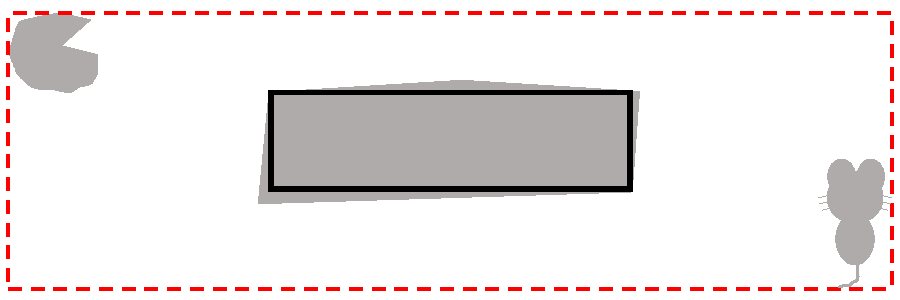
\includegraphics[width=3in]{fig.pdf}
\caption{Example where the underlying distribution $p$ is uniform over the (gray) valid regions. The solid rectangle maximizes our objective since it does not output nonsense (is supported only within the grey matter) and is closest to the $p$ (covers the maximum amount of grey matter). In contrast, the standard maximum likelihood (dashed red) rectangle must fully contain the observed samples, thus generating invalid points most of the time.  }
\end{figure}

Motivated by these observations, we evaluate a generative model $q$ on two axes. First is {\em coverage}, which is related to the probability assigned to future examples drawn from the true distribution $p$. Second is {\em validity}, defined as the probability that random examples generated from $q$ meet some validity requirement. Formally, we measure coverage in terms of a bounded {\em loss}:
$$\Loss(p,q)=\E_{x \sim p}[L(q_x)],$$
where $L:[0,1]\rightarrow [0,M]$ is a bounded decreasing function such as the capped log-loss $L(q_x)=\min(M, \log 1/q_x)$. % or $L(q_x)=\log 1/(q_x+\exp(-M))$. 
A bounded loss has the advantages of being efficiently estimable, and also it enables a model to assign 0 probability to one example (e.g., an outlier or error) if it greatly increases the likelihood of all other data. Validity is defined with respect to a set $V \subseteq X$, and $q(V)$ is the probability that a random example generated from $q$ lies within $V$. 

Clearly, there is a tradeoff between coverage and validity. We first focus on the case of (near) perfect validity. A Valid Generative Modeling (VGM) algorithm if it outputs, for a family of distributions $Q$ over $X$, if it outputs $\hat{q}$ with (nearly) perfect validity and whose loss is nearly as good as the loss of the best valid $q\in Q$. More precisely, $A$ is a VGM learner of $Q$ if for any nonempty valid subset $V \subseteq X$, any probability distribution $p$ over $V$, and any $\eps>0$, $A$ uses $n$ random samples from $p$ and makes $m$ membership oracle calls to $V$ and outputs a distribution $\hat{q}$ such that, $$\Loss(p, \hat{q}) \leq \min_{q \in Q: q(V)=1}\Loss(p,q) + \eps ~\text{ and }~\hat{q}(V)\geq 1-\eps.$$ 
We aim for our learner to be sample and query efficient, requiring that $n$ and $m$ are polynomial in $M, 1/\eps$ and a measure of complexity of our distribution class $Q$.
Furthermore, we would like our algorithms to be computationally efficient, with a runtime polynomial in the size of the data, namely the $n + m$ training examples. 
A more formal description of the problem is available in Section~\ref{sec:problem}.

$A$ is said to be {\em proper} if it always outputs $\hat{q}\in Q$ and {\em improper} otherwise.
In Section~\ref{sec:impossibility}, we first show that efficient proper learning for VGM is impossible. This is an information-theoretic result, meaning that even given infinite runtime and positive samples, one still cannot solve the VGM problem. Interestingly, this is different from binary classification, where it is possible to statistically learn from iid examples without a membership oracle.

Our first main positive result is an efficient (improper) learner for VGM. The algorithm relies on a subroutine that solves the following {\em Generative Modeling with Negatives} (GMN) problem: given sets $X_P, X_N \subset X$ of positive and negative examples, find the probability distribution $q \in Q$ which minimizes $\sum_{x \in X_P} L(q(x))$ subject to the constraint that $q(X_N)=0$. For simplicity, we present our algorithm for the case that the distribution family $Q$ is finite, giving sample and query complexity bounds that are logarithmic in terms of $|Q|$. However, as we show in Section~\ref{sec:infinite-families}, all of our results extend to infinite families $Q$. It follows that if one has a computationally efficient algorithm for the GMN problem for a distribution family $Q$, then our reduction gives a computationally efficient VGM learning algorithm for $Q$.

Our second positive result is an algorithm that minimizes $\Loss(p,q)$ subject to a relaxed validity constraint comparing against the optimal distribution that has validity $q(V)$ at least $1-\alpha$ for some $\alpha>0$. We show in Section~\ref{sec:partial-validity} that even in this more general setting, it is possible to obtain an algorithm that is statistically efficient but may not be computationally efficient. An important open question is whether there exists a computationally efficient algorithm for this problem when given access to an optimization oracle, as was the case for our algorithm for VGM.

\subsection{Related Work}
\cite{KearnsMRRSS94} showed how to learn distributions from positive examples in the realizable setting, i.e., where the true distribution is assumed to belong to the class being learned. In the same sense as their work is similar to PAC learning \citet{Valiant84} of distributions, our work is like agnostic learning \citet{KearnsSS94} in which no assumption on the true distribution is made. 

Generative Adversarial Networks (GANs)~\cite{GoodfellowPMXWOCB14} are an approach for generative modeling from positive examples alone, in which a generative model is trained against a discriminator that aims to distinguish real data from generated data. In some domains, GANs have been shown to outperform other methods at generating realistic-looking examples. Several shortcomings of GANs have been observed \citet{AroraRZ18}, and GANs are still subject to the theoretical limitations we argue are inherent to any model trained without a validity oracle. 

In supervised learning, there is a rich history of learning theory with various types of queries, including membership which are not unlike our (in)validity oracle. Under various assumptions, queries have been shown to facilitate the learning of complex classes such as finite automata \citet{Angluin88} and DNFs \citet{Jackson97}. See the survey of \cite{Angluin92} for further details.  Interestingly, \cite{Feldman09} has shown that for agnostic learning, i.e., without making assumptions on the generating distribution, the addition of membership queries does not enhance what is learnable beyond random examples alone. 
Supervised learning also has a large literature around active learning, showing how the ability to query examples reduces the sample complexity of many algorithms. See the survey of \cite{Hanneke14}. Note that the aim here is typically to save examples and not to expand what is learnable.
 
More sophisticated models, e.g., involving neural networks, can mitigate the invalidity problem as they often generate more realistic natural language and have even been demonstrated to generate \LaTeX{} that nearly compiles \citep{Karpathy15} or nearly valid Wikipedia markdown. However, longer strings generated are unlikely to be valid. For example, \cite{Karpathy15} shows generated markdown which includes:
\begin{quote}
==Access to ''rap===
The current history of the BGA has been [[Vatican Oriolean Diet]], British Armenian, published in 1893.  While actualistic such conditions such as the [[Style Mark Romanians]] are still nearly not the loss.
\end{quote}

Even ignoring the mismatched quotes and equal signs, note that this example has two so-called ``red links'' to two pages that do not exist. Without checking, it was not obvious to us whether or not Wikipedia had pages titled {\em Vatican Oriolean Diet} or {\em Style Mark Romanians}. In some applications, one may or may not want to disallow red links. In the case that they are considered valid, one may seek a full generative model of what might plausibly occur inside of brackets, as the neural network has learned in this case. If they are disallowed, a model might memorize links it has seen but not generate new ones. A validity oracle can help the learner identify what it should avoid generating.

 In practice, \cite{KusnerPH17} discuss how generative models from neural networks (in particular autoencoders) often generate invalid sequences. 
\cite{JanzWPKH18} learn the validity of examples output by a generative model using oracle feedback. 


%\section{Related Work} \label{sec:related}


Mixtures of Linear Regressions is a popular mixture model (e.g.,~\citep{de1989mixtures,grun2007applications} and \citep{faria2010fitting}), also known as Hierarchical Mixture of Experts in~\citep{jordan1994hierarchical} in the machine learning community. 
It has many applications, such as trajectory clustering~\citep{gaffney1999trajectory} and phase retrieval~\citep{balakrishnan2017statistical}, and has as special cases some popular models, such as piecewise linear regression and locally linear regression.

Learning MLR in general is NP-hard~\citep{yi2014alternating}. Recent interests have been in providing various efficient algorithms for recovering the parameters in MLR under assumptions about the data generation model~\citep{chaganty2013spectral,chen2014convex,yi2014alternating,zhong2016mixed,klusowski2017estimating}. 
%These results assumes the data $x$ in different components are all from the standard Gaussians. 
They are either under restricted assumptions about the data (mixtures of two component or $x$ all from the standard Gaussian)~\citep{chen2014convex,yi2014alternating,balakrishnan2017statistical,klusowski2017estimating}, or have high sample or computational complexity~\citep{chaganty2013spectral,sedghi2016provable}. 

Some works study specific algorithms for the problem, such as  the Expectation Maximization (EM) algorithm~\citep{khalili2007variable,yi2014alternating,balakrishnan2017statistical,klusowski2017estimating}. It is known that without careful initialization EM is only guaranteed to have local convergence~\citep{klusowski2017estimating}. A grid search method for initialization is proposed in~\citep{yi2014alternating} but is only for the two-component case. It is unclear how to generalize these guarantees to our more general setting where the data $x$ from different components are from different Gaussians.
Moreover, EM also often suffers from a high computational cost.
%, for example, exact optimization in each EM step has $O(d^2 N + d^3)$ complexity. 

Another line of works used tensor methods for MLR~\citep{chaganty2013spectral,sedghi2016provable}. The third-order moment is directly estimated in~\citep{chaganty2013spectral} using samples from Gaussian distribution and is estimated from a linear regression problem in~\citep{sedghi2016provable}. A significant drawback of tensor methods is high sample and computational complexity, due to the high cost in estimating and operating over the tensors. 

\citep{chen2014convex} provided a convex relaxation formulation and showed that their algorithm is information-theoretically optimal. However, it is only for the two-component case and suffers from high computational cost in nuclear norm minimization. 

\citep{zhong2016mixed} provided a non-convex objective function that is locally strongly convex in the neighborhood of the ground truth, and proposed to first use a tensor method for initialization and then optimize the provided objective, achieving a global convergence guarantee. The overall algorithm is fixed parameter tractable in the number of components, and achieves nearly optimal sample and time complexity when this parameter is constant. However, it requires all components have the standard Gaussian distribution. It is unclear how to generalize the result to our more general setting where the data $x$ from different components are from different Gaussians. Furthermore, due to the tensor initialization, the algorithm needs complicated assumptions on the moments, while our only essential assumption is that the weight parameters can be separated, which is much simpler and more general (in fact, it is essentially necessary for obtaining any recovery guarantees).

\citep{yi2016solving} gives an improved way of using the tensor method plus alternative minimization so the sample complexity linearly depend on $d$. However, their algorithm  requires that all the data are from the standard Gaussian, and the sample complexity also depends on the minimal singular value of certain moment matrix, which can be $ \Delta^{\Omega(k)}$ small in our setting. 


\newcommand{\lcomp}{\loss^{\circ}}
\section{Preliminaries}\label{s:prel}
%
We start by considering a nonstochastic multiarmed bandit problem on
$K$ actions with oblivious losses in which the loss $\loss_t(i) \in
[0,1]$ at time $t$ of an action $i \in \{1,\ldots, K\}$ is defined
by the sum
\[
  \loss_t(i) = \sum_{s=0}^{d-1} \loss_t^{(s)}(i)
\]
of $d$-many components $\loss_t^{(s)}(i) \ge 0$ for $s=0,\dots,d-1$.
Let $I_t$ denote the action chosen by the player at the
beginning of round $t$. If $I_t = i$, then the player incurs loss
$\loss_t^{(0)}(i)$ at time $t$, loss $\loss_t^{(1)}(i)$ at time $t+1$,
and so on until time $t+d-1$.
Yet, what the player observes at time $t$ is only the combined loss incurred at time $t$, which is the sum
$
\loss_{t}^{(0)}(I_{t}) + \loss_{t-1}^{(1)}(I_{t-1}) + \cdots + \loss_{t-d+1}^{(d-1)}(I_{t-d+1})
$
of the past $d$ loss contributions, where $\loss_t^{(s)}(i) = 0$ for all $i$ and $s$ when $t \le 0$. Since the setting $d=1$ recovers the standard nonstochastic oblivious bandit model, in the following we assume $d \ge 2$. For all sequences of actions $i_1, \ldots, i_d \in \{1,\ldots,K\}$, define the $d$-delayed {\em composite} loss function
%
\begin{equation}\label{e:mixedloss}
    \lcomp_t(i_1,i_2,\dots,i_d) = \sum_{s=0}^{d-1} \loss_{t-s}^{(s)}(i_{d-s})~,
\end{equation}
%
with $\loss_t^{(s)}(i) = 0$ for all $i$ and $s$ when $t \le 0$. With this notation, the $d$-delayed composite anonymous feedback assumption states that what the player observes at the end of each round $t$ is only the composite loss
$
\lcomp_t(I_{t-d+1},I_{t-d+2},\dots,I_t)
$.
Note that, whereas the losses $\loss_t(i)$ are in $[0,1]$, the composite loss can take values as large as $d$. On the other hand, the cumulative composite loss of any action $i$ over $d$ consecutive steps is at most $2d-1$:
\begin{equation}
\label{eq:compsum}
    \sum_{\tau=t-d+1}^t \lcomp_{\tau}(i,\dots,i)
=\!\!\!
    \sum_{\tau=t-d+1}^t \sum_{s=0}^{d-1} \loss_{\tau-s}^{(s)}(i)
\leq\!\!\!
    \sum_{\tau=t-2d+2}^t \sum_{s=0}^{d-1}\loss_{\tau}^{(s)}(i)
=\!\!\!
    \sum_{\tau=t-2d+2}^t \loss_{\tau}(i)
\le
    2d-1~.
\end{equation}
The goal of the algorithm is to bound its regret $R_T$ against the best fixed action in hindsight,
\[
R_T =\E\left[\sum_{t=1}^T \lcomp_t(I_{t-d+1},\dots,I_t)\right] -
\min_k \sum_{t=1}^T \lcomp_t(k,\dots,k)~.
\]
We define the regret in terms of the composite losses $\lcomp_t$ rather than the true losses $\loss_t$ because in our model $\lcomp_t$ is what the algorithm pays overall in round $t$. It is easy to see that a bound on $R_T$ implies a bound on the more standard notion of regret $\E\left[\sum_{t=1}^T \loss_t(I_t)\right] - \min_{k}\sum_{t=1}^T \loss_t(k)$ up to an additive term of at most $d-1$.
%\begin{align*}
%   \E\left[\sum_{t=1}^T \loss_t(I_t)\right] - \min_{k = 1,\ldots,K}\sum_{t=1}^T \loss_t(k)
%&=
%   \E\left[\sum_{t=1}^T \lcomp_t(I_{t-d+1},\dots,I_t)\right] - \sum_{t=1}^T \lcomp_t(k,\dots,k)
%   + \sum_{t=T-d+2}^T \sum_{s=T-t+1}^{d-1} \Big(\E\big[\loss_t^{(s)}(I_t)\big] - \loss_t^{(s)}(k)\Big)
%\\&\le
%   \E\left[\sum_{t=1}^T \lcomp_t(I_{t-d+1},\dots,I_t)\right] - \sum_{t=1}^T \lcomp_t(k,\dots,k) + (d-1)~.
%\end{align*}

Our setting generalizes the composite loss function setting of \citet{ddkp14}.
Specifically, the linear composite loss function therein can be seen as a
special case of the composite loss~(\ref{e:mixedloss}) once we remove
the superscripts $s$ from the loss function components. In fact, in the linear case,
the feedback in \citep{ddkp14} allows one to easily reconstruct each individual
loss component in a recursive manner. This is clearly impossible in our more
involved scenario, where the new loss components that are observed in round $t$ need
not have occurred in past rounds.


\newcommand{\blhat}{\widehat{\bloss}}
\newcommand{\bmu}{\boldsymbol{\mu}}
\newcommand{\bq}{\boldsymbol{q}}
\section{Wrapper Algorithm for Composite Losses}
\label{s:wrapper}
%
Our ``Composite Loss Wrapper'' algorithm (Algorithm~\ref{a:delayed-app}) wraps a standard bandit algorithm called here Base MAB (Base Multi-Armed Bandit). Base MAB operates on standard (noncomposite) losses with values in $[0,1]$,
producing probability distributions $\bp_t$ over the action set $\{1,\ldots,K\}$. The wrapper, which has access to a sequence
$B_0,B_1,\dots$ of i.i.d.\ Bernoulli random variables of parameter $q$ (to be chosen later), experiences three kinds of online rounds: a {\em draw}, an {\em update}, and a {\em stay}
round. If round $t$ is a draw round, the algorithm draws action $I_t$ according to the current distribution $\bp_t$
maintained by Base MAB, but without having Base MAB update $\bp_t$. If $t$ is an update round, then the algorithm's
action $I_t$ is the same as $I_{t-1}$ (in particular, the algorithm does not draw $I_t$ from $\bp_t$), but then a
distribution update $\bp_t \rightarrow \bp_{t+1}$ takes place by invoking the update rule of Base MAB over an
average of the observed losses.
Finally, if $t$ is a stay round, then both $I_t = I_{t-1}$ and $\bp_{t+1} = \bp_{t}$. The way these three
kinds of rounds are interleaved is illustrated in Figure~\ref{f:1}.
%
%% ----------------------------------------------------------------------------
\begin{algorithm2e}[t]
\SetKwSty{textrm} \SetKwFor{For}{{\bf For}}{}{}
\SetKwIF{If}{ElseIf}{Else}{if}{}{else if}{else}{}
\SetKwFor{While}{while}{}{}
\textbf{Input:}  Base MAB algorithm $A$ with parameter $\eta \in (0,1]$.\\%, and meta-parameters for it $\xi$.\\
\textbf{Initialize:}
\begin{itemize}[topsep=0pt,parsep=0pt,itemsep=0pt]
\item Draw $I_0$ from the uniform distribution $\bp_1$ over $\{1,\ldots,K\}$;
\item If $B_0 = 1$ then $t=0$ is an update round.
\end{itemize}
%
\For{$t=1,2,\dots$:} { {
\begin{enumerate}[topsep=0pt,parsep=0pt,itemsep=0pt]
\item If $t-1$ was an update round, then draw $I_t \sim \bp_t$ and play it without updating $\bp_t$ (draw round, $\bp_{t+1} = \bp_t$);
\item Else if an update round was in the interval $\{t-2d+1, \dots,t-2\}$ then play $I_t = I_{t-1}$ without updating $\bp_t$
(stay round, $\bp_{t+1} = \bp_t$);
\item Else play $I_t = I_{t-1}$ (stay round), and if $B_t=1$ then the stay round becomes an update round. In such a case:
%
\begin{minipage}{\textwidth-50pt}
\begin{itemize}
\vspace{0.05in}
\item Feed Base MAB $A(\eta)$ with average composite loss\footnote
{
Recall that when $t \leq 0$, we defined $\ell^{(s)}_{t} =0$, so the initial stretch of $2d-2$ actions $I_1,\ldots,I_{2d-2}$ can be disregarded here at the price of an extra additive $\scO(d)$ regret in the analysis.
}
%
\[
\avgloss_t = \frac{1}{2d}\sum_{\tau=t-d+1}^t \lcomp_\tau(I_{\tau-d+1},\dots,I_{\tau})
\]
\item Use the update rule $\bp_t\rightarrow \bp_{t+1}$ of Base MAB to obtain the new distribution $\bp_{t+1}$.
%(the stay round becomes an update round).
\end{itemize}
\end{minipage}
\end{enumerate}
%\vspace{-0.2in}
} } \caption{The Composite Loss Wrapper.}
\label{a:delayed-app}
\end{algorithm2e}
%% ---------------------------------------------------------------------------
%
\begin{figure}[t!]
\begin{picture}(-40,290)(-40,290)
\scalebox{0.7}{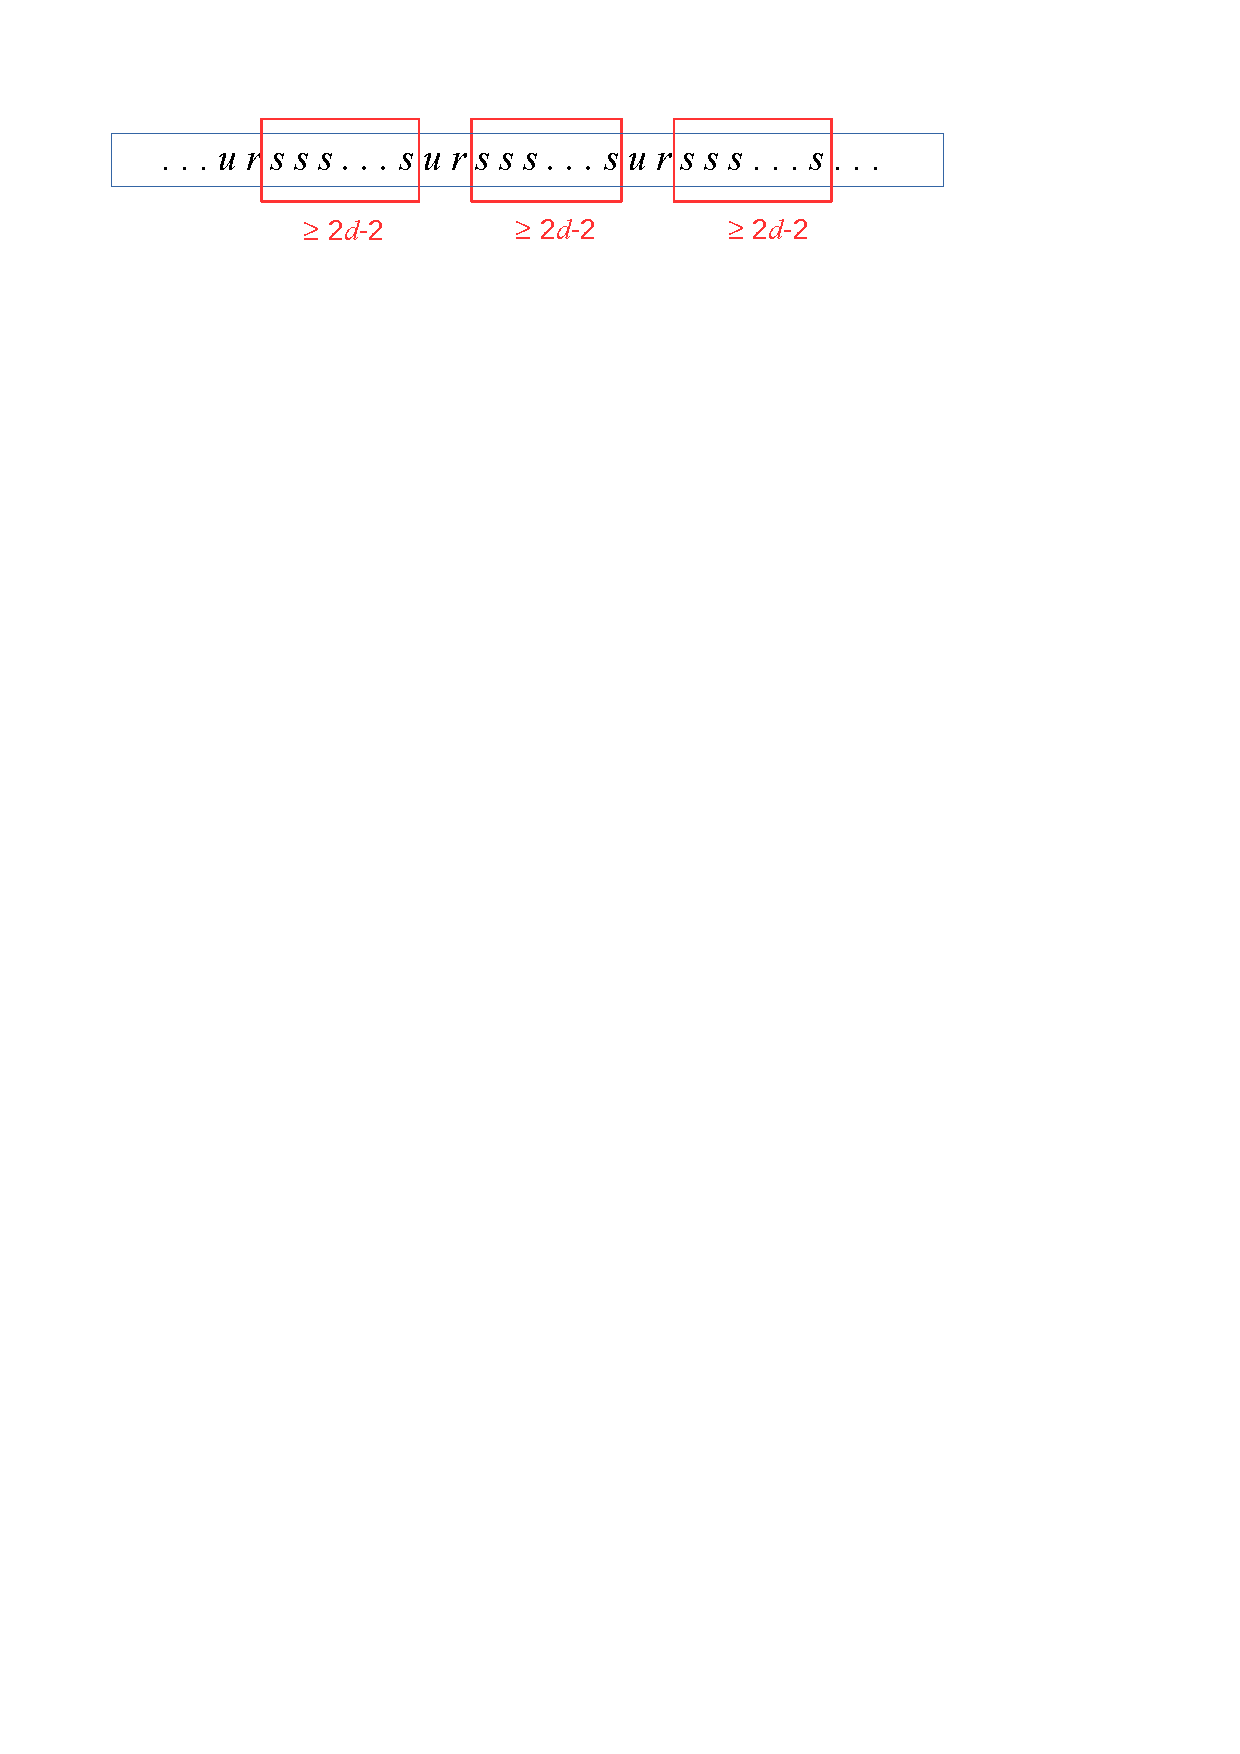
\includegraphics{interleave.pdf}}
\end{picture}
\vspace{-3.0in}
\caption{\label{f:1}
Sequence of rounds the algorithm is undergoing. Each ({\em u})pdate round is always followed by a d({\em r})aw round,
and then by a stretch of ({\em s})tay rounds whose length is random, but is at least $2d-2$.
The actual length of the stay stretch is ruled by the realizations of the Bernoulli random variables $B_t$.
}
\end{figure}


%%% ----------------------------------------------------------------------------
%\begin{algorithm2e}[t]
%\SetKwSty{textrm} \SetKwFor{For}{{\bf For}}{}{}
%\SetKwIF{If}{ElseIf}{Else}{if}{}{else if}{else}{}
%\SetKwFor{While}{while}{}{}
%\textbf{Parameter:} $\eta \in [0,1]$.\\
%\textbf{Initialize:}
%\begin{itemize}
%\item Draw $I_0$ from the uniform distribution $p_1$;
%\item If $B_0 = 1$ then $t=0$ is an update round.
%\end{itemize}
%%
%\For{$t=1,2,\dots$:}
%{ {
%\begin{enumerate}
%\item If $t-1$ was an update round, then draw $I_t \sim p_t$ and play it without updating $p_t$ (draw round);
%\item Else if $d > 2$ and an update round was in the interval $\{t-d+1, \dots,t-2\}$ then play $I_t = I_{t-1}$ without updating $p_t$
%(stay round);
%\item Else play $I_t = I_{t-1}$ (stay round), and if $B_t=1$ then perform an Exp3$(\eta)$ update of $p_t$
%using $\loss_t(I_t,\dots,I_{t-d+1})$ (the stay round becomes an update
%round).
%\end{enumerate}
%
%\vspace{-0.2in}
%} }
%\caption{Delayed Loss Algorithm}
%\label{a:delayed}
%\end{algorithm2e}
%%% ----------------------------------------------------------------------------
%%
%
Note that the algorithm's pseudocode corresponds to the description in Figure~\ref{f:1} in that update and draw rounds are interleaved,
and an update round is immediately followed by a draw round. If an update round occurs at time $t \ge 1$, then no update round
can occur during the next $2d-1$ rounds; the next update takes place at time $t+2d+G$ where $G \ge 0$ is a Geometric random variable
with parameter $q$. Hence a stretch of stay rounds is $2d-2+G$ round long.
Moreover,
\begin{itemize}[topsep=0pt,parsep=0pt,itemsep=0pt]
\item
If $t$ is not a draw round (i.e., it is either an update or a stay round), then the last action is played again.
\item
If $t$ is an update round, then we are guaranteed that $I_t=\cdots=I_{t-2d+1}$, since the last draw could have only occurred
at time $t-2d+1$ or earlier.
\end{itemize}
%
In order for our analysis to go through, we make mild assumptions on Base MAB. The first assumption (fulfilled by many
standard $K$-armed bandit algorithms ---see below) is a stability condition described in the following definition.
%
\begin{definition}\label{d:stabilityexp3}
Let $A(\eta)$ be a Base MAB with learning rate $\eta$,
and $\{\bp_t\}_{t=1}^T$ be the sequence of probability distributions over actions $\{1,\ldots,K\}$ produced by $A(\eta)$ during a run over $T$ rounds. We say that $A(\eta)$ is $\xi$-{\em stable} if for any round $t$ we have that
\[
    \E\left[\sum_{i\,:\,p_{t+1}(i) > p_t(i)} p_{t+1}(i) - p_t(i)\right] \leq \xi
\]
% deterministically
holds, where $\xi = \xi(K,\eta,\ldots)$ is a function of $K$, $\eta$, and possibly other relevant parameters of the Base MAB.
\end{definition}
%
The second assumption is that $A(\eta)$ is {\em nontrivial} for any $\eta > 0$:
when operating in the standard (non-delayed) bandit setting, $A(\eta)$ enjoys a concave (possibly linear) regret bound as a function of the time
horizon $T$.  Specifically, if we let $R_A(T,K,\eta)$ be a regret bound for $A$ when the time horizon is $T$, the number
of actions is $K$ and the learning rate is $\eta$, we have for any $K \geq 1$ and $\eta > 0$ that
%$R_A(T,K,\eta) = o(T)$ as $T \rightarrow \infty$, being
$R_A(T,K,\eta)$ is a concave function of $T$. For example,
$R_A(T,K,\eta) = \scO((\ln K)/\eta + \eta K T)$, which is linear in
$T$.
%
\iffalse
*********************************
Our algorithm receives a general Multi-Arm Bandit algorithm $A$,
which has a learning rate parameter $\eta$ and a set of hyper
parameters $\xi$. We will assume that MAB is {\em stable}, namely,
it does not change the action distribution by more than $2\eta$
between successive rounds. Formally, the definition of stable is the
following.
%
\begin{definition}
A MAB algorithm $A$ with parameter $\eta$ is {\em stable} if for any
history $h$ and loss $\ell$: it outputs the distribution $p$ after
$h$ and the distribution $p'$ after $h$ followed by $\ell$, then
$\|p-p'\|_1\leq 2\eta$
\end{definition}
%
The regret bound of a MAB algorithm $A$ with parameters $\eta$ and
$\xi$ is denoted by $R_A(T,K,\eta,\xi)$. Namely, for any sequence of
losses $\ell_t$ and any fixed action $j$ we have,
\[
\E[\sum_{t=1}^T \ell_t(a_t)]\leq \E[\sum_{t=1}^T \ell_t(j)] + R_A(T,K,\eta,\xi)
\]
where the expectation is over the probabilities that $A$ selects
action $a_t$ at time $t$.

We also assume that for any random variable ${\cal T}$ we have
\[
\E[R_A({\cal T},K,\eta,\xi)]\leq R_A(\E{\cal T},K,\eta,\xi)
\]
*********************************
\fi
We have the following theorem, whose proof is in the appendix.
%
\begin{theorem}\label{thm:delay-generic}
Let $A(\eta)$ be a $\xi$-stable and nontrivial Base MAB algorithm with learning rate $\eta$ and regret bound
$R_A(T,K,\eta)$ for standard $K$-armed bandits. Then
Algorithm~\ref{a:delayed-app} with input $A(\eta)$ achieves regret
\[
R_T \le T\,\xi + 8(2d-1)R_A(T/2d,K,\eta) + \scO(d)
\]
for $K$-armed bandits with $d$-delayed composite anonymous feedback.
%In particular, for $\eta = \sqrt{\frac{d\ln K}{TK}}$ we have a
%cumulative regret of $O(\sqrt{dTK\ln K} )$
\end{theorem}
%
%
%%%%%%%%%%%%%%%%%%%%%%%%%%%%%%%
%
We can now derive corollaries for various algorithms using Theorem~\ref{thm:delay-generic}. Consider for instance, the well-known
Exp3 algorithm of \citet{AuerCeFrSc02}. When operating with losses, the algorithm maintains a probability distribution
$\bp_t = (p_t(1),\ldots,p_t(K))$ over $\{1,\ldots,K\}$ of the form $p_t(i) = w_t(i)/\sum_{j=1}^K w_t(j)$, while the update rule
$\bp_t\rightarrow \bp_{t+1} $ can be described as follows:
\begin{equation}
\label{eq:expW}
w_{t+1}(i) = p_t(i)\,e^{-\eta\ellhat_t(i)},\quad \ellhat_t(i) = \frac{\ell_t(i)\Ind{I_t = i}}{p_t(i)},\quad i = 1, \ldots, K~.
\end{equation}
When the losses $\ell_t(i)$ are in $[0,1]$ we have the regret bound
\(
R_{\mathrm{Exp3}}(T,K,\eta) \leq \frac{\ln K}{\eta}+\frac{\eta}{2}\,K\,T~.
\)
Moreover, the following simple stability property holds (proof in the appendix).
%
\begin{lemma}\label{l:stabilityexp3}
Exp3 with learning rate $\eta$ is $\xi$-stable with $\xi = \eta$.
\end{lemma}
%
Combined with Theorem~\ref{thm:delay-generic}, this implies the following regret bound with composite losses.
%
\sloppypar{
\begin{corollary}\label{c:delay-generic}
%With the notation introduced so far,
If Algorithm~\ref{a:delayed-app} is run with Exp3($\eta$) with $\eta = 4\sqrt{\frac{d\,\ln K}{(4K+1)\,T}}$ as Base MAB, then its regret for $K$-armed bandits with $d$-delayed composite anonymous feedback satisfies
\[
R_T \leq 8\sqrt{d\,(4K+1)\,T\,\ln K} + \scO(d) = \scO(\sqrt{dKT\ln K})~.
\]
\end{corollary}
}
%
$K$-armed bandits are a special case of combinatorial linear bandits
\citep{cesa2012combinatorial}, a setting where actions are incidence
vectors $\bv\in\scK\subset\bool^n$ describing elements in some
combinatorial space (e.g., spanning trees of a given graph) and loss
vectors $\bloss_t \in [0,1]^n$ satisfy $\bloss_t^{\top}\bv \in
[0,1]$ for all $\bv\in\scK$ (in $K$-armed bandits, $\scK$ is simply
the canonical basis of $\bool^n$). Let $\bv_t\in\scK$ be the action
played at time $t$. The generalization of Exp3 for the combinatorial
bandit setting uses the Exp2 algorithm with loss estimates of the
form $\blhat_t = P_t^+ \bv_t \bv_t^{\top} \bloss_t$, where $P_t =
\E_{\bV \sim \bp_t}\bigl[\bV \bV^{\top}\bigr]$ and $P_t^+$ is the
pseudo inverse of $P_t$ ---see \citep{dani2008price}. Note that
these estimates are unbiased: $\E_t\big[\blhat_t^{\top}\bv] =
\bloss_t^{\top}\bv$ for all $\bv\in\scK$. The distribution $\bp_t$
is a mixture $\bp_t = (1-\gamma)\bq_t + \bmu$, where $0 < \gamma <
1$, $\bq_t$ has the exponential form~(\ref{eq:expW})
\[
    q_t(\bv) = \frac{w_t(\bv)}{\sum_{\bv'\in\scK} w_t(\bv')}~,
\quad
    w_{t+1}(\bv)
=
    q_t(\bv)\,e^{-\eta\,\blhat_t^{\top}\bv}~,
\quad
    \bv\in\scK~,
\]
and $\bmu$ is a fixed exploration distribution on $\scK$. When run with an appropriate exploration distribution $\bmu$ and $\gamma = \eta n < 1$, Exp2$(\eta)$ has the following regret bound ---see, e.g., \citep[Theorem~4]{bubeck2012towards},
$
    R_{\mathrm{Exp2}}(T,\scK,\eta) \le \big(\ln|\scK|\big)\big/{\eta} + 3\eta nT
$.
Now, similarly to Lemma~\ref{l:stabilityexp3}, we can prove the following (the proof is provided in the appendix):
%
\begin{lemma}
\label{l:stabExp2}
Exp2 with learning rate $\eta$ and mixing coefficient $\gamma$ is $\xi$-stable with $\xi = (1-\gamma)\eta$.
\end{lemma}
%
Combining again with Theorem~\ref{thm:delay-generic}, the above implies the following regret bound with composite losses.
%
\begin{corollary}
\label{c:delayExp2}
If Algorithm~\ref{a:delayed-app} is run with Exp2($\eta$) with $\eta = 4\sqrt{\frac{d\,\ln|\scK|}{(24n+1)\,T}}$ as Base MAB, then its regret for $\scK$-combinatorial bandits, $\scK \subseteq \{0,1\}^n$, with $d$-delayed composite anonymous feedback satisfies
\[
    R_T
\le
    8\sqrt{d\,(24n+1)\,T\,\ln|\scK|} + \scO(d) = \scO(\sqrt{dnT\ln|\scK|})~.
\]
\end{corollary}
%
\begin{remark}\label{r:firstorderbound}
The proof of Lemma~\ref{l:stabilityexp3} in the appendix shows pointwise stability, a stronger notion than the expected stability of Definition~\ref{d:stabilityexp3}. In fact, an outer expectation over the random variable $I_t$ in the proof of Lemma~\ref{l:stabilityexp3} makes the stability parameter $\xi$ be upper bounded by $\eta\sum_{i=1}^K p_{t}(i)\ell_{t}(i)$ in round $t$, so that the term $T\xi$ in Theorem~\ref{thm:delay-generic} can be replaced by $\eta\,L_A(T)$, where $L_A(T)$ is the cumulative (average) loss of the Base MAB. Coupled with a ``first order" regret analysis of Exp3 where $T$ is indeed replaced by $L_A(T)$ ---see~\citep[Theorem~2]{allenberg2006hannan}, this gives a regret bound in the composite anonymous feedback setting where $T$ is likewise replaced by $L_A(T)$.
\end{remark}


\newcommand{\Rlin}{R^{\mathrm{lin}}}
\section{Lower bound}
\label{s:lower}
In this section we derive a lower bound for bandits with composite anonymous feedback. We do that through a reduction from the setting of linear bandits (in the probability simplex) to our setting. This reduction allows us to upper bound the regret of a linear bandit algorithm in terms of (a suitably scaled version of) the regret of an algorithm in our setting. Since the reduction applies to any instance of a linear bandit problem, we can use a known lower bound for the linear bandit setting to derive a corresponding lower bound for our composite setting.

Let $\Delta_K$ be the probability simplex in $\R^K$. At each round $t$, an algorithm $A$ for linear bandit optimization chooses an action $\bp_t\in\Delta_K$ and suffers loss $\bloss_t^{\top}\bp_t$, where $\bloss_t \in [0,1]^K$ is some unknown loss vector. The feedback observed by the algorithm at the end of round $t$ is the scalar $\bloss_t^{\top}\bp_t$. The regret suffered by algorithm $A$ playing actions $\bp_1,\dots,\bp_T$ is
\begin{equation}
\label{eq:lin-regret}
	\Rlin_T = \sum_{t=1}^T \bloss_t^{\top}\bp_t - \min_{\bp\in\Delta_K} \sum_{t=1}^T \bloss_t^{\top}\bp = \sum_{t=1}^T \bloss_t^{\top}\bp_t - \min_{i=1,\dots,K} \sum_{t=1}^T \loss_t(i)
\end{equation}
where we used the fact that a linear function on the simplex is minimized at one of the corners.
Let $\Rlin_T(A,\Delta_K)$ denote the worst case regret (over the oblivious choice of $\bloss_1,\dots,\bloss_T$) of algorithm $A$. Similarly, let $R_T(A_d,K,d)$ be the worst case regret (over the oblivious choice of loss components $\loss_t^{(s)}(i)$ for all $t$, $s$, and $i$) of algorithm $A_d$ for nonstochastic $K$-armed bandits with $d$-delayed composite anonymous feedback. Our reduction shows the following.
%
\begin{lemma}\label{lem:lower}
For any algorithm $A_d$ for $K$-armed bandits with $d$-delayed composite anonymous feedback, there exists an algorithm $A$ for linear bandits in $\Delta_K$ such that
$
	R_T(A_d,K,d) \ge d\,\Rlin_{T/d}(A,\Delta_K)
$.
\end{lemma}
%
%
Our reduction, described in detail in the proof of the above lemma (see the appendix), essentially builds the probability vectors $\bp_t$ played by $A$ based on the empirical distribution of actions played by $A_d$ during blocks of size $d$. Now, an additional lemma is needed (whose proof is given in the appendix).
\begin{lemma}
\label{l:shamir}
The regret of any algorithm $A$ for linear bandits in the simplex satisfies $\Rlin_T(A,\Delta_K) = \widetilde{\Omega}\big(\sqrt{KT}\big)$.
\end{lemma}
%
Using the above two lemmas we can prove the following theorem.
\begin{theorem}
For any algorithm $A_d$ for $K$-armed bandits with $d$-delayed composite anonymous feedback,
$
R_T(A_d,K,d)=\widetilde{\Omega}\big(\sqrt{dKT}\big)
$.
\end{theorem}
%
\begin{proof}
Fix an algorithm $A_d$. Using the reduction of~Lemma~\ref{lem:lower} gives an algorithm $A$ such that
$
	R_T(A_d,K,d) \ge d\,\Rlin_{T/d}(A,\Delta_K) = \widetilde{\Omega}\big(\sqrt{dKT}\big)
$,
where we used Lemma~\ref{l:shamir} with horizon $T/d$ to prove the $\widetilde{\Omega}$-equality.
\end{proof}
%
Although the loss sequence used to prove the lower bound for linear bandits in the simplex is stochastic i.i.d., the loss sequence achieving the lower bound in our delayed setting is not independent due to the deterministic loss transformation in the proof of Lemma~\ref{lem:lower} (which is defined independent of the algorithm, thus preserving the oblivious nature of the adversary).



%\section{Discounted loss}

Assume that the losses are discounted by some parameter $\gamma
\in(0,1)$ rather than bounded by $d$. Namely,
\[
    \loss_t(I_{1},\dots,I_t) = \sum_{s=0}^{t-1} \loss_{t-s}^{(s)}(I_{t-s})\gamma^{t-s} (1-\gamma)
\]
Note that if for any $\tau$, $s<\tau$ and action $i$ we have
$\loss_{\tau}(i)^{(s)}\in [0,1]$ then we have that
$\loss_t(I_{1},\dots,I_t)\in[0,1]$.

We can run the same algorithm and assume that we have
$d=2\log_\gamma T$, i.e., $\gamma^d=T^{-2}$. We have that
\[
\sum_{s=0}^{t-1} \loss_{t-s}^{(s)}(I_{t-s})\gamma^{t-s} (1-\gamma) -
\sum_{s=0}^{d-1} \loss_{t-s}^{(s)}(I_{t-s})\gamma^{t-s} (1-\gamma)
\leq \frac{1}{T^2}
\]
the two loss sequences should behave very similar. [[YM: I recall we
had problems with the discounted setting, but I cannot reconstruct
them now. Is the issue only the $\log T$ factor in the regret?]]


%% !TeX root = main.tex
\section{Extensions}
\label{sec:extensions}

% !TeX root = main.tex
\subsection{Partial validity}
\label{sec:partial-validity}
In this section, we consider a generalization of our main setting, where we allow some slack in the validity constraint.
More precisely, given some parameter $\alpha > 0$, we now have the requirement that $\Loss(\hat q) \leq \Loss(q^*) + \eps_1$ and $\Inv(\hat q) \leq \alpha + \eps_2$, where $q^*$ is the optimal distribution which minimizes $\Loss(q^*)$ such that $\Inv(q^*) \leq \alpha$.

%In this result, we allow points to be ``partially valid'' -- specifically, we let $\Inv: X \rightarrow [0,1]$ take fractional values.

\subsubsection{Algorithm}
We provide an algorithm for solving the partial validity problem in Algorithm~\ref{alg:partial-validity}.
This method is sample-efficient, requiring a number of samples which is $\poly\left(M, \eps_1^{-1}, \eps_2^{-1}, \log |Q|\right)$.

\begin{algorithm}[ht]
   \caption{Learning a distribution with partial validity}
   \label{alg:partial-validity}
\begin{algorithmic}[1]
   \STATE {\bfseries Input:} Sample and invalidity access to a distribution $p$, parameters $\ve_1, \ve_2, \alpha > 0$, a family of distributions $Q$.
   \STATE Using $n_1$  samples from $p$, empirically estimate $\overline \Loss(q) \in \Loss(q) \pm \frac {\eps_1} 3$ for all $q \in Q.$
   \FOR{$\ell \in \left\{0, \frac {\eps_1} 3,..., M\right\}$} \label{ln:partial-validity-outer-loop}
   \STATE Let $D = \{q \in Q\ |\ \overline \Loss(q) \le \ell \}$.
   \STATE Let $x^*$ be any point with $\Inv(x^*) = 0$.
   \STATE Let $\mu_D$ be the distribution which samples a distribution $q$ uniformly from $D$, and then draws a sample from $q$.
   \WHILE{$D \neq \emptyset$} \label{ln:partial-validity-inner-loop}
   \STATE Draw $n_2$ samples $x_1, ..., x_{n_2}$ from $\mu_D$.
   \IF {$\frac{1}{n_2} \sum_{i=1}^{n_2} \Inv(x_i) \Pr_{q \sim \Unif(D)}[q(x_i) {\eps_1} < 3 \mu_D(x_i)  {M} ] \le \alpha + \frac {4 \eps_2}{5}$}
   \RETURN $\mu'_D$, which samples $x$ from $\mu_D$ with probability $$\Pr_{q \sim \Unif(D)}[q(x) {\eps_1} < 3 \mu_D(x) {M} ],$$ and samples $x^*$ otherwise.
   \ELSE \STATE Remove all distributions $q$ from $D$ for which $$\frac{1}{n_2} \sum_{i=1}^{n_2} \Inv(x_i) \frac {q(x_i)} {\mu_D(x_i)} \Ind[q(x_i) {\eps_1} < 3 \mu_D(x_i) {M} ] > \alpha + \frac {\eps_2} {5}.$$  
   \ENDIF
   \ENDWHILE
   \ENDFOR
\end{algorithmic}
\end{algorithm}

\subsubsection{Analysis}
We will show that, with high probability, Algorithm~\ref{alg:partial-validity} outputs a distribution $\hat q$ that has $\Loss(\hat q) \leq \Loss(q^*) + \eps_1$ and $\Inv(\hat q) \leq \alpha + \eps_2$.

\begin{theorem}\label{thm:partial-validity}
  Suppose that the loss function $L$ is convex.
  The choice of parameters
  \begin{equation}
  n_1 = \Theta\left(\frac{M^2}{\ve_1^2} \log |Q| \right), n_2 = \Theta\left(\frac {M^2} {\eps_1^2 \eps_2^2} \log |Q| \log \left(\frac{M \log |Q|}{\eps_1 \eps_2}\right)\right)
  \end{equation}
  guarantees that Algorithm~\ref{alg:partial-validity} outputs w.p. $3/4$ a distribution with $\Loss(\hat q) \le \Loss(q^*) + \eps_1$ and $\Inv(\hat q) \le \alpha + \eps_2$ using $\Theta\left(\frac{M^2}{\ve_1^2} \log |Q| \right)$ samples from $p$ and $\Theta\left(\frac{M^3}{ \ve_1^3 \ve_2^3} \log^2 |Q| \log \left(\frac{M \log |Q|}{\eps_1\eps_2}\right)\right)$ invalidity queries.
\end{theorem}

\begin{remark}
We note that this algorithm still works in the case where points may be ``partially valid'' -- specifically, we let $\Inv: X \rightarrow [0,1]$ take fractional values.
This requires that we have access to some point $x^*$ where $\Inv(x^*) = 0$, which we assume is given to us by some oracle.
For instance, the distribution may choose to output a dummy symbol $\bot$, rather than output something which may not be valid. 
\end{remark}

We prove Theorem~\ref{thm:partial-validity} through three lemmas.
The sample complexity bound follows from the values of $n_1$, $n_2$, the fact that we have at most $O\left(\frac{M}{\eps_1}\right)$ iterations of the loop at Line~\ref{ln:partial-validity-outer-loop}, and Lemma~\ref{lem:partial-validity-inner-loop} which bounds the number of iterations of the loop at Line~\ref{ln:partial-validity-inner-loop} as $O\left(\frac{\log |Q|}{\eps_2}\right)$ for any $\ell$.
To argue correctness, Lemmas~\ref{lem:partial-validity-invalid} and~\ref{lem:partial-validity-loss} bound the invalidity and loss of any output distribution, respectively.
The proofs of these lemmata appear in Section~\ref{sec:partial-proofs}.

\begin{lemma}
\label{lem:partial-validity-inner-loop}
With probability at least $14/15$, the loop at Line~\ref{ln:partial-validity-inner-loop} requires at most $O\left(\frac{\log |Q|}{\eps_2}\right)$ iterations for each $\ell$.
\end{lemma}

\begin{lemma}
\label{lem:partial-validity-invalid}
With probability at least $14/15$, if at any step a distribution $\mu'_D$ is output, $\Inv(\mu'_D) \le \alpha + \eps_2$.
\end{lemma}

\begin{lemma}
\label{lem:partial-validity-loss}
With probability at least $14/15$, if at any step a distribution $\mu'_D$ is output, $\Loss(\mu'_D) \le \ell + 2\eps_1/3$, where $\ell$ is the step at which the distribution was output.
\end{lemma}

The proof of Theorem~\ref{thm:partial-validity} concludes by observing that the optimal distribution $q^*$ is never eliminated (assuming all estimates involving its loss and validity are accurate, which happens with probability at least $19/20$), and that the loop in line~\ref{ln:partial-validity-outer-loop} steps by increments of $\eps_1/3$. 
Combining this with Lemma~\ref{lem:partial-validity-loss}, if we output $\hat q$, then $\Loss(\hat q) \leq \Loss(q^*) + \eps_1$.

\newcommand{\fat}{s}
\newcommand{\vc}{d}

\subsection{General Densities}
\label{sec:densities}

For simplicity of presentation, we have formulated the above results in terms of probability mass functions $q$ on a discrete domain $X$.
However, we note that all of the above results easily extend to general density functions on an abstract measurable space $X$, which 
may be either discrete or uncountable.  Specifically, if we let $\mu_{0}$ denote an arbitrary reference measure on $X$, 
then we may consider the family $Q$ to be a set of \emph{probability density functions} $q$ with respect to $\mu_{0}$: that is, 
non-negative measurable functions such that $\int q {\rm d}\mu_{0} = 1$.  
For the results above, we require that we have a way to (efficiently) generate iid samples having the distribution whose density is $q$.
For the full-validity results, the only additional requirements are that we are able to (efficiently) test whether a given $x$ is in the support of $q$,
and that we have access to $\text{Oracle}(\cdot,\cdot)$ defined with respect to the set $Q$.
For the results on partial-validity, we require the ability to explicitly evaluate the function $q$ at any $x \in X$.
The results then hold as stated, and the proofs remain unchanged (overloading notation to let $q_{x}$ denote the 
value of the density $q$ at $x$, and $q(A) = \int_{A} q {\rm d}\mu_{0}$ the measure of $A$ 
under the probability measure whose density is $q$).

\subsection{Infinite Families of Distributions}
\label{sec:infinite-families}

%%% maybe no space to define VC-dim and fat-shattering dim, but we can at least give references for both.

It is also possible to extend all of the above results to \emph{infinite} families $Q$, 
expressing the sample complexity requirements in terms of the \emph{VC dimension} (\cite{VapnikC74}) of the supports $\vc = {\rm VCdim}(\{\Supp(q) : q \in Q\})$, 
and the \emph{fat-shattering dimension} (\cite{AlonBCH97}) of the family of loss-composed densities $\fat(\epsilon) = {\rm fat}_{\epsilon}(\{ x \mapsto L(q_{x}) : q \in Q \})$.
In this case, in the context of the full-validity results, 
for simplicity we assume that in the evaluations of $\text{Oracle}(X_{P},X_{N})$ defined above, 
there always \emph{exists} at least one minimizer $q \in Q$ of the empirical loss with respect to $X_{P}$ 
such that $\Supp(q) \cap X_{N} = \emptyset$.\footnote{It is straightforward to remove this assumption by supposing 
$\text{Oracle}(X_{P},X_{N})$ returns a $q$ that \emph{very-nearly} minimizes the empirical loss, and handling 
this case requires only superficial modifications to the arguments.}
We then have the following result.  For completeness, we include a full proof in the appendix.

\begin{theorem}
\label{thm:vc-full-validity}
For a numerical constant $c \in (0,1]$, 
the choice of parameters 
\begin{eqnarray*}
P=\Theta\left(\frac{\fat(c \ve_{1}/M) M^{2}}{\ve_1^2} \log \frac{M}{\ve_{1}} \right), & R = \Theta \left( \frac { M } {\eps_1} \right), &  T = \Theta\left(\frac{R \vc}{\ve_2} \log \frac{1}{\ve_{2}} \right)
\end{eqnarray*}
guarantees that Algorithm~\ref{alg:full-validity} outputs w.p. $3/4$ a distribution $\hat q$ with $\Loss(\hat q) \le \Loss(q^*) + \eps_1$ and $\Inv(\hat q) \le \eps_2$ 
using $P$ samples from $p$ and $R T$ invalidity queries.
  
The algorithm runs in time polynomial in $M$, $\ve_1^{-1}$, $\ve_2^{-1}$, $\vc$, and $\fat_{\ve_{1}/256}$ assuming that queries to the optimization oracle 
can be computed in polynomial time. Moreover, sampling from the resulting distribution $\hat q$ can also be performed in polynomial time.
\end{theorem}

For partial-validity, we can also extend to infinite $Q$, 
though in this case via a more-cumbersome technique.
Specifically, let us suppose the densities $q \in Q$ are bounded by $1$ (this can be replaced by any value by varying the sample size $n_2$).
Then we consider running Algorithm~\ref{alg:partial-validity} as usual, 
except replacing Step 4 with the step 
\begin{equation*}
D = {\rm Cover}_{\ve_{2}}( \{ q \in Q | \overline\Loss(q) \leq \ell \} ),
\end{equation*} 
where for any $R \subseteq Q$, ${\rm Cover}_{\ve_{2}}(R)$ denotes a minimal subset of $R$ such that 
$\forall q \in R$, $\exists q^{\ve_{2}} \in {\rm Cover}_{\ve_{2}}(R)$ with $\int | q_{x} - q^{\ve_{2}}_{x} | \mu_{0}({\rm d}x) \leq \ve_{2}$:
that is, an $\ve_{2}$-cover of $R$ under $L_{1}(\mu_{0})$.
Let us refer to this modified algorithm as Algorithm~\ref{alg:partial-validity}$^{\prime}$.
%Now denote by $\fat_{Q}(\epsilon) = {\rm fat}_{\epsilon}(Q)$.
We have the following result. 

\begin{theorem}
\label{thm:vc-partial-validity}
Suppose that the loss function $L$ is convex.
For a numerical constant $c \in (0,1]$, 
the choice of parameters
\begin{eqnarray*}
n_1 = \Theta\left(\frac{\fat(c\ve_{1}/M) M^{2}}{\ve_1^2} \log \!\left(\frac{M}{\ve_{1}}\right)  \right), & n_2 = \Theta\left(\frac {M^2 {\rm fat}_{c\ve_{2}}(Q)} {\ve_1^2 \ve_2^2} \log^{2} \!\left(\frac{M {\rm fat}_{c\ve_{2}}(Q)}{\ve_1 \ve_2}\right)\right)
\end{eqnarray*}
guarantees that Algorithm~\ref{alg:partial-validity}$^{\prime}$ (with parameters $\eps_{1}$, $\eps_{2}$, and $\alpha+\eps_{2}$) 
outputs w.p. $3/4$ a distribution with 
$\Loss(\hat q) \le \Loss(q^*) + \ve_1$ and $\Inv(\hat q) \le \alpha + 2\ve_2$ using $n_{1}$ samples from $p$ and 
$\Theta\left(\frac {M^3 {\rm fat}_{c\ve_{2}}(Q)^{2}} {\ve_1^3 \ve_2^3} \log^{3} \!\left(\frac{M {\rm fat}_{c\ve_{2}}(Q)}{\ve_1 \ve_2}\right)\right)$ 
invalidity queries.
\end{theorem}

% we'll assume, for simplicity, that there always is an empirical loss minimizer.  it just simplifies the arguments, but is pretty easy to extend to the general case by putting more \epsilon's all over the place.



\newcommand{\fcomp}{f^{\circ}}
\newcommand{\scD}{\mathcal{D}}
\newcommand{\bb}{\boldsymbol{b}}
\newcommand{\B}{\field{B}}

\section{Extensions: Bandit Convex Optimization}\label{s:bco}
%
We now show that a similar reduction as the one in Section~\ref{s:wrapper} can be made to work in the more general Bandit Convex Optimization (BCO) framework. This learning setting is defined by a convex and compact domain $\Omega \subseteq \R^n$ and a sequence of loss functions $f_1, f_2, \ldots, f_T$, where each $f_t\,:\,\Omega \to [0,1]$ is convex over $\Omega$. We assume each function $f_t$ is the cumulated effect of $d$-many convex loss components $f_t^{(0)},\ldots, f_t^{(d-1)}$, with $f_t^{(s)}\,:\,\Omega \to [0,1]$ so that, for any $\bw \in \Omega$,
%
\[
f_t(\bw) = \sum_{s=0}^{d-1} f_t^{(s)}(\bw) \in [0,1]~.
\]
To be concrete, we shall view $f_t$'s components $f_t^{(s)}$ as constant fractions of $f_t$, specifically,
\[
f_t^{(s)}(\bw) = \alpha^{(s)}_{t} f_t(\bw)~, \qquad s = 0,\ldots, d-1~, \qquad t = 1,\ldots, T\,,
\]
for nonnegative constant coefficients $\alpha^{(s)}_{t}$ such that $\sum_{s=0}^{d-1}\alpha^{(s)}_{t} =1$, for $t = 1, \ldots, T$.

Since we are working with oblivious adversaries, we assume that all losses $\{f_{t}\}_{t=1\dots T}$ and coefficients $\{\alpha^{(s)}_{t}\}_{t=1\dots T,s=0\dots d-1}$ are generated before the game starts. At each round $t= 1, 2, \ldots, T$, the learner picks $\tbw_t \in \Omega$ and suffers loss $f^{(0)}_t(\tbw_t) = \alpha^{(0)}_{t}f_t(\tbw_t)$ at time $t$, loss $f^{(1)}_{t}(\tbw_t) =  \alpha^{(1)}_{t} f_{t}(\tbw_t)$ at time $t+1,\ldots,$ loss $f^{(d-1)}_t(\tbw_t) =  \alpha^{(d-1)}_{t}f_t(\tbw_t)$ at time $t+d-1$. However, what the algorithm really observes at time $t$ is the cumulated effect of present and past actions quantified by the composite loss
\(
\fcomp_t(\tbw_{t-d+1},\tbw_{t-d+2},\ldots, \tbw_t)
\)
with
\[
\fcomp_t(\bw_{1},\bw_{2},\ldots, \bw_d)= \sum_{s=0}^{d-1} f_{t-s}^{(s)}(\bw_{d-s}) = \sum_{s=0}^{d-1} \alpha_{t-s}^{(s)}\,f_{t-s}(\bw_{d-s})~,
\]
where in the above $\alpha_t^{(s)} = 0$ for all $s$ if $t \leq 0$.
The aim of the algorithm is to minimize its regret
\[
% R_T = \E\left[\sum_{t=1}^T f_t(\tbw_{t})\right] - \min_{\bw \in \Omega} \sum_{t=1}^T f_t(\bw)~.
    R_T =\E\left[\sum_{t=1}^T \fcomp_t(\tbw_{t-d+1},\dots,\tbw_t)\right] - \min_{\bw} \sum_{t=1}^T \fcomp_t(\bw,\dots,\bw)~.
\]
As in previous sections, we build a wrapper around a base Bandit Convex Optimization algorithm (Base BCO) which operates in the standard BCO framework with standard losses with range in $[0,1]$. Base BCO maintains at each round $t$ a state variable $\bw_t$ which is randomly perturbed to obtain the actual play $\tbw_t \in \Omega$. The wrapper algorithm is described as Algorithm~\ref{a:delayed-bco}.
%
%% ----------------------------------------------------------------------------
\begin{algorithm2e}[t]
\SetKwSty{textrm} \SetKwFor{For}{{\bf For}}{}{}
\SetKwIF{If}{ElseIf}{Else}{if}{}{else if}{else}{}
\SetKwFor{While}{while}{}{}
\textbf{Input:} Base BCO algorithm $A$ with parameter $\eta \in (0,1]$.\\%, and meta-parameters for it $\xi$.\\
\textbf{Initialize:}
\begin{itemize}[topsep=0pt,parsep=0pt,itemsep=0pt]
\item Play any $\bw_1 \in \Omega$;
\item If $B_0 = 1$ then $t=0$ is an update round.
\end{itemize}
%
\For{$t=1,2,\dots$:} { {
\begin{enumerate}[topsep=0pt,parsep=0pt,itemsep=0pt]
\item If $t-1$ was an update round, then play $\tbw_t$ by randomly perturbing state variable $\bw_t$ without updating $\bw_t$ (draw round, $\bw_{t+1} = \bw_t$);
\item Else if an update round was in the interval $\{t-2d+1, \dots,t-2\}$ then play $\tbw_t = \tbw_{t-1}$ without updating $\bw_t$
(stay round, $\bw_{t+1} = \bw_t$);
\item Else play $\tbw_t = \tbw_{t-1}$ (stay round), and if $B_t=1$ then the stay round becomes an update round. In such a case:
%
\begin{minipage}{\textwidth-50pt}
\begin{itemize}[topsep=0pt,parsep=0pt,itemsep=0pt]
\vspace{0.05in}
\item Feed Base BCO $A(\eta)$ with average composite loss\footnote
{
Recall that when $t \leq 0$, we defined $\alpha^{(s)}_{t} =0$, for all $s$, so the initial stretch of $2d-2$ actions $\tbw_1,\ldots,\tbw_{2d-2}$ can be disregarded here at the price of an extra additive $\scO(d)$ regret in the analysis.
}
%
\[
\avglossf_t = \frac{1}{2d}\sum_{\tau=t-d+1}^t \fcomp_\tau(\tbw_{\tau-d+1},\dots,\tbw_{\tau})
\]
\item Use the update rule $\bw_t\rightarrow \bw_{t+1}$ of Base BCO to obtain the new state variable $\bw_{t+1}$.
%(the stay round becomes an update round).
\end{itemize}
\end{minipage}
\end{enumerate}
%\vspace{-0.2in}
} } \caption{The Composite Loss Wrapper for BCO.}
\label{a:delayed-bco}
\end{algorithm2e}
%% ----------------------------------------------------------------------------
%
The notion of stability of the Base BCO has now to refer also to the sequence of loss functions the algorithm is operating with. Notice that, unlike the standard notion of stability in Online Convex Optimization, the kind of stability we need here is a {\em backward} stability, for it involves the backward differences $f_{t+1}(\tbw_{t+1}) - f_{t+1}(\tbw_t)$, rather than the forward differences $f_{t}(\tbw_{t}) - f_{t}(\tbw_{t+1})$. Moreover, we have to consider only the positive part of the backward difference.
%
\begin{definition}\label{d:stabilitybco}
Let $A(\eta)$ be a Base BCO with learning rate $\eta$, and $\{\tbw_t\}_{t=1}^T$ be the sequence of plays produced by $A(\eta)$ during a run over $T$ rounds on the sequence of convex losses $\{f_t\}_{t=1}^T$. We say that $A(\eta)$ is $\xi$-{\em stable} w.r.t.\ $\{f_t\}_{t=1}^T$ if for any round $t$ we have that\footnote
{
Here and throughout, $[x]_+ = \max\{x,0\}$. The outer $[\cdot]_+$ in Definition \ref{d:stabilitybco} forces $\xi$ to be nonnegative. 
}
\[
    \Bigl[\E\Big[f_{t+1}(\tbw_{t+1}) -f_{t+1}(\tbw_t) \Big]\Bigl]_+ \leq \xi
\]
% deterministically
holds, where $\xi$ may depend on the input dimension $n$, the learning rate $\eta$, as well as on relevant properties of the loss functions $\{f_t\}_{t=1}^T$ and parameters of the algorithm.
\end{definition}
%
We call a Base BCO algorithm $A$ {\em nontrivial} w.r.t.\ the sequence of losses $\{f_t\}_{t=1}^T$ if, when applied to the standard setting on $\{f_t\}_{t=1}^T$, $A$ has a regret bound $R_A(T,n,\eta)$ which is concave (possibly linear) in $T$ for any $n \geq 1$, $\eta > 0$, and the other relevant parameters of the algorithm.
%
Theorem~\ref{thm:convex} below rests on the assumption that the properties of the loss functions $\{f_t\}_{t=1...T}$ that make the Base BCO algorithm $A$ work are inherited by the average composite loss functions
%
\begin{align*}
\avglossf_t(\bw) &= \frac{1}{2d}\sum_{\tau=t-d+1}^t \fcomp_\tau(\bw,\dots,\bw)~, \qquad {\mbox{for $t \geq 2d-2$}},
\end{align*}
%
the wrapper feeds to $A$. For the sake of concreteness, let us simply focus on boundedness, Lipschitzness, and $\beta$-smoothness w.r.t. the Euclidean norm $||\cdot||$. Recall that a convex function $f\,:\,\Omega \to [0,1]$ is said to be $\beta$-smooth (or, equivalently, to have $\beta$-Lispchitz continuous gradient) w.r.t.\ $||\cdot||$ if for all $\bw, \bw' \in \Omega$ we have $||\nabla f(\bw) - \nabla f(\bw')|| \leq \beta ||\bw-\bw'||$, where $\beta \geq 0$. Moreover, given constants $\beta_1,\beta_2, b_1, b_2 \geq 0$, if $f_1$ is $\beta_1$-smooth w.r.t.\ $||\cdot||$ and $f_2$ is $\beta_2$-smooth w.r.t.\ $||\cdot||$, then it is easy to see that $b_1 f_1 + b_2 f_2$ is ($b_1\beta_1+b_2\beta_2$)-smooth w.r.t.\ $||\cdot||$. The following proposition lists the relevant properties of the functions $\avglossf_t$ as immediate consequences of the properties of the functions $f_t$ (proven in the appendix).
%
\begin{proposition}\label{l:propcomposite}
Let $f_1,\ldots, f_T\,:\,\Omega \subseteq \R^n \to [0,1]$ be a sequence of convex loss functions, and $\avglossf_{2d-2}, \ldots, \avglossf_T \,:\,\Omega \subseteq \R^n \to \R^+$ be the corresponding sequence of average composite losses. Then the following holds.
\begin{enumerate}[topsep=0pt,parsep=0pt,itemsep=0pt]
\item
$
\avglossf_{t}(\bw) \in [0,1]
$ for all $\bw \in \Omega$~.
\item If, for some constant $L \geq 0$, the loss functions $f_1,\ldots, f_T$ are $L$-Lipschitz on $\Omega$ w.r.t.\ $||\cdot||$, then so are $\avglossf_{2d-2},\ldots, \avglossf_T$.
\item If, for some constant $\beta \geq 0$, the loss functions $f_1,\ldots, f_T$ are $\beta$-smooth w.r.t.\ $||\cdot||$, then so are $\avglossf_{2d-2},\ldots, \avglossf_T$.
\end{enumerate}
\end{proposition}
%
The following theorem, whose proof sketch is in the appendix, is the BCO counterpart to Theorem~\ref{thm:delay-generic}.
%
%\ncb{Define properties P.}
\begin{theorem}\label{thm:convex}
Let $A(\eta)$ be a $\xi$-stable and nontrivial Base BCO algorithm with learning rate $\eta$ and regret bound
$R_A(T,n,\eta)$ in the standard BCO setting on a sequence of convex losses $\{f_t\}_{t=1}^T$ enjoying Properties $P$ (e.g., a subset of those listed in Proposition \ref{l:propcomposite}). If Properties $P$ are inherited by $\{\avglossf_t\}_{t=2d-2}^T$~, then Algorithm~\ref{a:delayed-bco} with input $A(\eta)$ achieves regret $R_T$ satisfying
\[
R_T
\le
T\,\xi + 8(2d-1)R_A(T/2d,n,\eta)+\scO(d)~.
  %  2T\eta + 4(2d-1)\left(\frac{\ln K}{\eta} + \frac{\eta}{4d}KT\right)~.
\]
\end{theorem}
%
%
As an example, consider the Base BCO algorithm by \citet{st11} that works under the assumption of $\beta$-smoothness w.r.t.\ $||\cdot||$. This algorithm is a BCO variant of the SCRIBLe algorithm by \citet{ahr12}. The algorithm takes in input a learning rate $\eta$, a scaling parameter $\delta \in (0,1]$ (which will be set as a function of $\eta$), and a $\nu$-self-concordant (barrier) function $\Psi$ which we assume to be strongly convex w.r.t. $||\cdot||$. For instance, if $\Omega$ is defined by a set of $m$ linear constraints $\Omega = \{\bw \in \R^n\,:\, A\bw \leq b \}$, a standard choice of $\Psi$ is the sum of negative log distances to each boundary, i.e., $\Psi(\bw) = -\sum_{i=1}^m \log(b_i - \be_i^\top A\bw)$, where $b = (b_1,\ldots, b_m)^\top$, and $\be_i$ is the $i$-th unit vector in the canonical basis of $\R^m$. Then $\Psi$ is strongly convex w.r.t.\ $||\cdot||$, up to a strong convexity constant. The algorithm maintains at each round $t$ the state variable $\bw_t \in \Omega$, of the form
%
\begin{equation}\label{e:st11}
\bw_t = \argmin_{\bw\in \Omega}\ \eta\,\sum_{\tau = 1}^{t-1} \bw^\top{\hat g_{\tau}} + \Psi(\bw)~.
\end{equation}
%
Then, it computes a perturbed version $\tbw_t$ of $\bw_t$ as
\(
\tbw_t = \bw_t + \delta H_t^{-1/2}\,s_t~,
\)
where $H_t$ is the Hessian matrix $\nabla^2 \Psi(\bw_t)$, $s_t$ is drawn uniformly at random from the surface of the Euclidean $n$-dimensional unit ball $\B^n$, and $\delta = \delta(\eta) \in (0,1]$ is a scaling parameter. Finally, the update $\bw_t \rightarrow \bw_{t+1}$ amounts to computing the next vector ${\hat g_{t}}$ in~(\ref{e:st11}) as ${\hat g_{t}} = \frac{n}{\delta}\,f_t(\tbw_t)H_t^{1/2}s_t$,
% \citet{st11} show that the vector ${\hat g_{t}}$ is
an unbiased estimate of the gradient at $\bw_t$ of a smoothed version
%${\hat f_t}$
of $f_t$.
%, defined as
%\(
%{\hat f_t}(\bw) = \E_{b\sim \B^n} [f(\bw+\delta H_t^{-1/2} b)]~,
%\)
%where $b$ is drawn uniformly at random from $\B^n$.
From \citep{st11} one can bound $R_A(T,n,\eta) = R_A(T,n,\eta,\delta(\eta))$ as follows:
%
\begin{equation}\label{e:st11bound}
R_A(T,n,\eta) \leq \beta T\delta^2\scD^2 + \eta T\left(\frac{n}{\delta}\right)^2 + \frac{2\nu\log T}{\eta} + \left(\frac{2}{\scD} + \scD\beta\right)\sqrt{T}~,
\end{equation}
%
where $\scD = \max_{\bw,\bw'\in \Omega} ||\bw-\bw'||$ is the diameter of $\Omega$. Moreover, the following stability lemma can be shown (proven in the appendix).
%
\begin{lemma}\label{l:stabilityconvexscrible}
Let $f_1,\ldots,f_T\,:\,\Omega \subseteq \R^n \rightarrow [0, 1]$ be a sequence of $\beta$-smooth convex losses w.r.t. $||\cdot||$, and $\scD$ be the diameter of $\Omega$. Then the Base BCO algorithm by \cite{st11} is $\xi$-stable, with
$
\xi = \scO\left(\left(1/\scD + \scD\beta\right)\frac{\eta\,n}{\delta}  + \beta\delta^2\scD^2\right)
$.
\end{lemma}
%
Combining~(\ref{e:st11bound}) with Theorem~\ref{thm:convex} and Lemma~\ref{l:stabilityconvexscrible} implies the following regret bound for composite losses.
%
\begin{corollary}\label{c:st11}
If Algorithm~\ref{a:delayed-bco} is run with the abovementioned algorithm by \citet{st11} as Base BCO algorithm, with $\eta = \scO\left(\left(\frac{d\log (T/d)}{n\,T}\right)^{2/3}\right)$ and $\delta = \scO(\eta^{1/4}\,n^{1/2})$, then its regret for BCO with $d$-delayed composite anonymous feedback satisfies
$
R_T = \scO\left(\bigl(d\log (T/d)\bigl)^{1/3}\,(n\,T)^{2/3} + \sqrt{d\,T}\right)
$,
where the $\scO$ notation in the tuning of $\eta,\delta$ and in the bound on $R_T$ hides the constants $\beta$, $\scD$ and $\nu$.
\end{corollary}
%
\begin{remark}
A similar statement can be made in the special case of bandit linear optimization, where the losses $f_t$ are $\beta$-smooth with $\beta =0$. In this case, Corollary \ref{c:st11} with $\delta = 1$ and $\eta$ set appropriately gives a bound of the form $\scO\left(\sqrt{d\,n^2\,T\,\log(T/d)}\right)$. The rate $T^{2/3}$ shown in Corollary~\ref{c:st11} is the same as the one achieved by the Base BCO algorithm of \citet{st11}. Likewise, the rate $T^{1/2}$ achieved by Corollary~\ref{c:st11} for the linear case is the same as the one obtained by the analyses in \citep{ahr12,st11}. In both cases (and in line with the results in Sections \ref{s:wrapper} and \ref{s:lower}) we have an extra factor $\sqrt{d}$ introduced by the composite anonymous feedback.
\end{remark}


%
\section{Conclusions}
%
We have investigated the setting of $d$-delayed composite anonymous feedback as applied to nonstochastic bandits. Composite anonymous feedback lends itself to formalize scenarios where the actions perfomed by the online decision maker produce long-lasting effects that combine additively over time. A general reduction technique was introduced that enables the convertion of a (backward stable) algorithm working in a standard bandit framework into one working in the composite feedback framework. 
In the case of $K$-armed bandits, we relied on a lower bound for bandit linear optimization in the probability simplex to show that no algorithm in the composite feedback framework can do better than $\scO(\sqrt{dKT})$. In turn, up to log factors, this is what we obtain as an upper bound by applying our reduction to the standard Exp3 algorithm.

We showed the generality and flexibility of our conversion technique by further applying it to Combinatorial Bandits (the Exp2 algorithm) and to Bandit Convex Optimization (the self-concordant barrier-based algorithms by \cite{ahr12} and \cite{st11}) with smooth/linear loss functions. In the latter case, the resulting Bandit Convex Optimization algorithm for composite anonymous feedback turned out to achieve regret bounds with higher rates than those of the corresponding base bandit algorithms, and we suspect that there is margin for improvement in our stability analysis of Lemma \ref{l:stabilityconvexscrible}.


\iffalse
************************
We then extended our results to the Bandit Convex Optimization framework, thereby showing the generality and flexibility of our conversion technique. As an example, we applied 

We Our reduction is flexible

 that works under the assumption of an oblivious adversary generating loss components. 

provided a general reduction that does such and such

in the case of k armed upper and lower bound, matching up to log factors. lower bound reduces to bandit linear optimization




flexibility, extension to combinatorial and bco, an example of application with beta smooth and self-concordant barriers.

Our analysis of bco is almost certainly suboptimal,
************************
\fi




\section{Conclusions}
%
We have investigated the setting of $d$-delayed composite anonymous feedback as applied to nonstochastic bandits.
% Composite anonymous feedback lends itself to formalize scenarios where the actions perfomed by the online decision maker produce long-lasting effects that combine additively over time.
A general reduction technique was introduced that enables the conversion of a (backward stable) algorithm working in a standard bandit framework into one working in the composite feedback framework. In the case of $K$-armed bandits, we relied on a lower bound for bandit linear optimization in the probability simplex to show that no algorithm in the composite feedback framework can do better than $\scO(\sqrt{dKT})$. In turn, up to log factors, this is what we obtain as an upper bound by applying our reduction to the standard Exp3 algorithm. We showed the generality and flexibility of our conversion technique by further applying it to Combinatorial Bandits (the Exp2 algorithm) and to Bandit Convex Optimization (the self-concordant barrier-based algorithms by \cite{ahr12} and \cite{st11}) with smooth/linear loss functions.

Three main directions for extending our work are:
\begin{itemize} 
\item Proving an upper bound for the case of nonoblivious adversaries;
\item Investigating the setting where the delay parameter $d$ is not perfectly known;
\item Extending our results to the nonstochastic contextual case.
\end{itemize}

\iffalse
 ****** CG: still working on it *****

In the latter case, the resulting Bandit Convex Optimization algorithm for composite anonymous feedback turned out to achieve regret bounds with higher rates than those of the corresponding base bandit algorithms, and we suspect that there is margin for improvement in our stability analysis of Lemma \ref{l:stabilityconvexscrible}.

Say something about possible directions
\fi


% Acknowledgments---Will not appear in anonymized version
\acks{YM was supported in part by a grant from the Israel Science
Foundation (ISF).}
\newpage

\bibliography{ncb}


\appendix
%





\section{Proof of Theorem \ref{thm:delay-generic}}

\begin{proof}
Let $\scU \subseteq \{1, \ldots, T\}$ be the (random) subset of update
rounds. Let us call for brevity an update round a $u$-round, and
similarly for the other two kinds. First, observe that if $t$ is a $u$-round, 
we have $\avgloss_t \in [0,1]$. This is because, due to~(\ref{eq:compsum}) and the fact that $I_t = I_{t-1} = \ldots = I_{t-2d+1}$,
%
\begin{align*}
	\avgloss_t 
=
	\frac{1}{2d}\sum_{\tau=t-d+1}^t \lcomp_\tau(I_{\tau-d+1},\dots,I_{\tau})
=
	\frac{1}{2d}\sum_{\tau=t-d+1}^t \lcomp_\tau(I_{t},\dots,I_{t})
\le
   \frac{1}{2d}(2d-1) < 1~.
\end{align*}
%
% First, observe that for any $t \in \scU$ we update using $loss_t$,
% where
%\[
% loss_t = \frac{1}{2d}\sum_{\tau=t-d}^t
% \loss_\tau(I_\tau,\dots,I_{\tau-d+1})\in[0,1]
% \]
% For $t\in \scU$ we have $I_t=\cdots=I_{t-2d+1}$, which implies that
% for any $\tau \in [t-2d+1,t]$ we have
% $\loss_\tau(I_{\tau-d+1},\dots,I_{\tau}) =
% \loss_\tau(I_{t-2d+1},\dots,I_{t-2d+1})$. So that
% \[
%     loss_t = \frac{1}{2d}\sum_{\tau=t-d}^t \sum_{s=0}^{d-1} \loss_{\tau-s}^{(s)}(I_{t-2d+1})\in[0,1]~.
% \]
%
Since a $u$-round is followed by an $r$-round, and during the stretch of $s$-rounds between an $r$-round 
and the next $u$-round the action played by Algorithm \ref{a:delayed-app} does not change, the algorithm
behaves exactly as $A(\eta)$ on the steps in $\scU$. Therefore, if we set for brevity
\[
\Delta_t^k = \frac{1}{2d}\sum_{\tau=t-d+1}^t \Big(\lcomp_\tau(I_{\tau-d+1},\dots,I_{\tau-d+1}) - \lcomp_\tau(k,\dots,k)\Big)~,
\qquad\text{for $t \geq 2d-2$},
\]
we have, for any action $k$,
%
\begin{equation}
\label{e:upperupdate}
	\E\left[\sum_{t \in \scU,\, t\geq 2d-2} \Delta_t^k\right]
\le 
	\E\big[R_A(|\scU|,K,\eta)\big] 
\le
	R_A\big(\E[|\scU|],K,\eta\big)
\le
	R_A(T/2d,K,\eta)~,
%    \le \frac{\ln K}{\eta} + \frac{\eta}{2}K\,\E\bigl[|\scU|\bigr] \le \frac{\ln K}{\eta} + \frac{\eta}{4d}KT
\end{equation}
%
where the second-last inequality is due to the concavity of $R_A(\cdot, K,\eta)$, and
the last inequality derives from $|\scU| \leq T/2d$, for there
can be at most one $u$-round every $2d$ rounds.
%({\bf CG:} I believe one can easily show $\E\bigl[|\scU|\bigr] \leq T/(3d)$ when $q=1/d$.)
Now, notice that by definition of a $u$-round we have, for all $t$,
\[
\Ind{t \in \scU} = \Ind{B_t = 1}\,\Ind{\bigwedge_{s=1}^{2d-1}(t-s\not\in \scU)}~.
\]
Moreover,
% if we set for brevity
% \[
% \Delta_t^k=\avgloss_t - \frac{1}{2d}\sum_{\tau=t-d+1}^t \loss_\tau(k,\dots,k)~,
% \]
% for $t \geq 2d-2$, we can write
%
\begin{align}
	\sum_{t=2d-2}^T \Delta_t^k 
&=
	\frac{1}{2d}\sum_{t=2d-2}^T\sum_{\tau=t-d+1}^t \Big( \lcomp_\tau(I_{\tau-d+1},\dots,I_{\tau-d+1}) - \lcomp_\tau(k,\dots,k) \Big)
\nonumber
\\&= 
	\frac{1}{2d}\sum_{t=d-1}^{2d-3} (t-d+2)\Big( \lcomp_t(I_{t-d+1},\dots,I_{t-d+1}) - \lcomp_t(k,\dots,k) \Big)
\nonumber
\\&
	\quad + \frac{d}{2d}\sum_{t=2d-2}^{T-d+1} \Big( \lcomp_t(I_{t-d+1},\dots,I_{t-d+1}) - \lcomp_t(k,\dots,k) \Big)
\nonumber
\\&
	\quad +\frac{1}{2d}\sum_{t=T-d+2}^{T} (T+1-t)\Big( \lcomp_t(I_{t-d+1},\dots,I_{t-d+1}) - \lcomp_t(k,\dots,k) \Big)
\nonumber
\\&\geq 
	\frac{1}{2}\sum_{t=2d-2}^{T-d+1} \Big( \lcomp_t(I_{t-d+1},\dots,I_{t-d+1}) - \lcomp_t(k,\dots,k) \Big)
\nonumber
\\&
	\quad - \frac{1}{2d}\sum_{t=d-1}^{2d-3} (t-d+2)\lcomp_t(k,\dots,k) - \frac{1}{2d}\sum_{t=T-d+2}^{T} (T+1-t)\lcomp_t(k,\dots,k)
\nonumber
\\&\ge
	\frac{1}{2}\sum_{t=2d-2}^{T-d+1} \Big( \lcomp_t(I_{t-d+1},\dots,I_{t-d+1}) - \lcomp_t(k,\dots,k) \Big) - 2(d-1)~,
\label{e:lowerdelta}
\end{align}
where the last inequality holds because, due to~(\ref{eq:compsum}),
\[
	\sum_{t=d-1}^{2d-3} (t-d+2)\lcomp_t(k,\dots,k) \le (d-1)\sum_{t=d-1}^{2d-3} \lcomp_t(k,\dots,k) \le (d-1)(2d-1)
\]
and
\[
	\sum_{t=T-d+2}^{T} (T+1-t)\lcomp_t(k,\dots,k) \le (d-1)\sum_{t=T-d+2}^{T} \lcomp_t(k,\dots,k) \le (d-1)(2d-1)~.
\]
Now, for any action $k$ we have,
\begin{align}
    \E&\left[\sum_{t \in \scU,\, t\geq 2d-2} \Delta_t^k \right]
=
    \E\left[\sum_{t=2d-2}^T \Ind{t \in \scU} \Delta_t^k \right]
\nonumber\\ &=
    \E\left[\sum_{t=2d-2}^T \Ind{B_t = 1}\,\Ind{\bigwedge_{s=1}^{2d-1}(t-s \not\in \scU)} \Delta_t^k \right]
\nonumber\\ &=
    q\,\E\left[\sum_{t=2d-2}^T \E\left[\Ind{\bigwedge_{s=1}^{2d-1}(t-s \not\in \scU)}\Delta_t^k \,\bigg|\, B_0,\dots,B_{t-2d},I_0,\ldots,I_{t-2d+1}
    \right]\right]
\nonumber\\ &=
    q\,\E\left[\sum_{t=2d-2}^T \Delta_t^k\,\E\left[\Ind{\bigwedge_{s=1}^{2d-1}(t-s \not\in \scU)} \,\bigg|\, B_0,\dots,B_{t-2d},I_0,\ldots,I_{t-2d+1}  \right]
    \right]
\nonumber\\ &=
    q\,\E\left[\sum_{t=2d-2}^T \Delta_t^k\,\E\left[\Ind{\bigwedge_{s=1}^{2d-1}(t-s \not\in \scU)} \,\bigg|\, B_0,\dots,B_{t-2d} \right]
     \right]
\nonumber\\ &=
    q\,\E\left[\sum_{t=2d-2}^T \Delta_t^k\,\Pr'\left(\bigwedge_{s=1}^{2d-1}(t-s \not\in \scU) \right)
     \right]\,,\label{e:expecteddelta}
\end{align}
where we set for brevity $\Pr'(\cdot) = \Pr\bigl(\,\cdot \mid
B_0,B_1\dots,B_{t-2d}\bigr)$.
%
We can thus write
%
\begin{align*}
    1 - \Pr'\left(\bigwedge_{s=1}^{2d-1}(t-s \not\in \scU) \right)
&=
    \Pr'\left(\bigvee_{s=1}^{2d-1}(t-s \in \scU) \right)
\\ &\le
    \sum_{s=1}^{2d-1}\Pr'\bigl(t-s \in \scU\bigr)
\\ & \le
    \sum_{s=1}^{2d-1}\Pr'\bigl(B_{t-s} = 1, t-s-1 \notin \scU, \ldots, t-s-2d+1 \notin \scU\bigr)
\\ & \le
    q\,(2d-1)\,.
\end{align*}
%
Hence, substituting into~(\ref{e:expecteddelta}) and combining with~(\ref{e:lowerdelta}), we conclude that
%
\begin{align}
	\E&\left[\sum_{t \in \scU,\,t\geq 2d-2} \Delta_t^k \right] 
\ge
	q(1-q(2d-1))\sum_{t=2d-2}^T \E\big[\Delta_t^k\big]
\nonumber
\\&\ge
    \frac{q}{2}(1-q(2d-1))\left( \sum_{t=2d-2}^{T-d+1} \Big(\E\big[\lcomp_t(I_{t-d+1},\dots,I_{t-d+1})\big] - \lcomp_t(k,\dots,k)\Big) - 2(d-1) \right)~.
     \label{e:updatenoupdate}
\end{align}
%
Next, using $\E_t[\cdot]$ to denote expectation conditioned on all random events at time steps $1,\dots,t-1$, we observe that
%
\begin{align}
\nonumber
    \E&\Bigl[ \lcomp_t(I_{t-d+1},\dots,I_t) - \lcomp_t(I_{t-d+1},\dots,I_{t-d+1}) \Bigr]
\\&=
\nonumber
    \E\left[ \sum_{s=0}^{d-1} \Bigl( \E_{t-s}\big[\loss_{t-s}^{(s)}(I_{t-s})\big] - \E_{t-d+1}\big[\loss_{t-s}^{(s)}(I_{t-d+1})\big] \Bigr)\right]
\\&=
\nonumber
    \E\left[ \sum_{s=0}^{d-1} \sum_{i=1}^K \loss_{t-s}^{(s)}(i) \bigl(p_{t-s}(i) - p_{t-d+1}(i)\bigr) \right]
\\&\le
\label{eq:stability} 
    \E\left[ \sum_{s=0}^{d-1} \sum_{i\,:\,p_{t-s}(i) > p_{t-d+1}(i)} \bigl(p_{t-s}(i) - p_{t-d+1}(i)\bigr) \right]
%\\ &\le
%    \sum_{s=0}^{d-1} \norm{\bp_{t-s} - \bp_{t-d+1}}_1
\le
    \xi~,
\end{align}
%
where the last inequality is because in any block of $2d$ rounds there is
at most one update of distribution $\bp_t$, each loss component $\loss_{t-s}^{(s)}(i)$ is in $[0,1]$, and because $A(\eta)$ is a $\xi$-stable 
Base MAB.
%update of $A$ changes the distribution by at most $2\eta$ in $1$-norm.
Hence we can write
\begin{align*}
	R_T
&\le
	\E\left[\sum_{t=1}^T \lcomp_t(I_{t-d+1},\dots,I_t)\right] - \sum_{t=1}^T \lcomp_t(k,\dots,k)
\\&=
	\E\left[\sum_{t=1}^T \lcomp_t(I_{t-d+1},\dots,I_t) - \sum_{t=1}^T \lcomp_t(I_{t-d+1},\dots,I_{t-d+1})\right]
\\&
	\quad + \E\left[\sum_{t=1}^T \lcomp_t(I_{t-d+1},\dots,I_{t-d+1})\right] - \sum_{t=1}^T \lcomp_t(k,\dots,k)
\\&\le
	T\,\xi + \underbrace{\E\left[\sum_{t=1}^T \lcomp_t(I_{t-d+1},\dots,I_{t-d+1})\right] - \sum_{t=1}^T \lcomp_t(k,\dots,k)}_{(\star)}
	\tag{from~(\ref{eq:stability})}
\end{align*}
%
Furthermore,
%
\begin{align*}
	(\star)
&\leq
	\E\left[\sum_{t=2d-2}^{T-d+1} \lcomp_t(I_{t-d+1},\dots,I_{t-d+1})\right] - \sum_{t=2d-2}^{T-d+1} \lcomp_t(k,\dots,k) + 3d
\\&\leq
	q(d-1) + \frac{2}{q(1-q(2d-1))}\,\E\left[\sum_{t\in \scU,\,t\geq 2d-2} \Delta_t^k \right] + 3d
\tag{from~(\ref{e:updatenoupdate})}
\\&\leq
	q(d-1) + \frac{2}{q(1-q(2d-1))}\,R_A(T/2d,K,\eta) + 3d~.
\tag{from~(\ref{e:upperupdate})}
\end{align*}
%
By picking $q = \tfrac{1}{2(2d-1)}$ so as to maximize the denominator in the second term of the right-most side yields
$
(*) \leq 8(2d-1)\,R_A(T/2d,K,\eta) + \scO(d)
$, 
so that
$
R_T \leq T\,\xi + 8(2d-1)\,R_A(T/2d,K,\eta) + \scO(d),
$
as claimed.
\end{proof}




\section{Proof of Lemma \ref{l:stabilityexp3}}
\begin{proof}
In this case, stability holds pointwise (for all realizations of $I_1,\dots,I_T$) rather that in expectation. From~\cite[Lemma 1]{cgmm16} we have, for any round $t$,
\[
	p_{t+1}(i) - p_t(i) \leq \eta\,p_{t+1}(i) \sum_{j=1}^K p_t(j) \ellhat_t(j)
\]
%
Hence we can write
%
\begin{align*}
\sum_{i\,:\,p_{t+1}(i) > p_t(i)} p_{t+1}(i)-p_t(i)
&\leq
\sum_{i\,:\,p_{t+1}(i) > p_t(i)} \eta\,p_{t+1}(i) \sum_{j=1}^K p_t(j) \ellhat_t(j)\\
&=
\sum_{i\,:\,p_{t+1}(i) > p_t(i)} \eta\,p_{t+1}(i) \ell_t(I_t)\\
&\leq
\eta\,\sum_{i\,:\,p_{t+1}(i) > p_t(i)} p_{t+1}(i)\\
&\leq
\eta
\end{align*}
concluding the proof.
\end{proof}



\section{Proof of Lemma \ref{l:stabExp2}}
%
\begin{proof}
Since $\bq_t$ has exponential form, we can apply again~\cite[Lemma 1]{cgmm16} and obtain
\[
	p_{t+1}(\bv) - p_t(\bv)
=
	(1-\gamma)\big(q_{t+1}(\bv) - q_t(\bv)\big)
\le
	(1-\gamma)\eta\,q_{t+1}(\bv) \sum_{\bv'\in\scK} q_t(\bv')\,\blhat_t^{\top}\bv'~.
\]
%
Hence we can write
%
\begin{align*}
	\E&\left[\sum_{\bv \,:\, p_{t+1}(\bv) > p_t(\bv)} p_{t+1}(\bv) - p_t(\bv) \right]
\\&\le
	(1-\gamma)\eta\,\E\left[\sum_{\bv \,:\, p_{t+1}(\bv) > p_t(\bv)} q_{t+1}(\bv) \sum_{\bv'\in\scK} q_t(\bv') \E_t\Big[\blhat_t^{\top}\bv'\Big] \right]
\\&=
	(1-\gamma)\eta\,\E\left[\sum_{\bv \,:\, p_{t+1}(\bv) > p_t(\bv)} q_{t+1}(\bv) \sum_{\bv'\in\scK} q_t(\bv') \bloss_t^{\top}\bv' \right]
	\tag{because estimates are unbiased}
\\&\le
	(1-\gamma)\eta\,\E\left[\sum_{\bv \,:\, p_{t+1}(\bv) > p_t(\bv)} q_{t+1}(\bv) \right]
	\tag{because $\bloss_t^{\top}\bv \in [0,1]$ for all $t$ and $\bv$}
\\&\le
	(1-\gamma)\eta
\end{align*}
concluding the proof.
\end{proof}



\section{Proof of Lemma \ref{lem:lower}}

\begin{proof}
Fix an algorithm $A_d$ for the $d$-delayed bandit setting. Given an assignment $\bloss_1,\dots,\bloss_{T/d}$ of loss vectors for the linear bandit setting, define, for each $i=1,\dots,K$, the loss components of the $d$-delayed bandit setting:
\[
	\loss_t^{(s)}(i) = \left\{ \begin{array}{cl}
		\loss_{\lceil t/d\rceil}(i) & \text{if $t+s\!\!\!\pmod d=0$,}
	\\[1mm]
		0 & \text{otherwise.}
	\end{array} \right.
\]
These components define the following composite loss for $A_d$ playing actions $I_t$,
\[
	\lcomp_t(I_{t-d+1},\dots,I_t)
=
	\sum_{s=0}^{d-1} \loss_{t-s}^{(s)}(I_{t-s})
=	
	\left\{ \begin{array}{cl}
		d\,\bp_t^{\top}\bloss_{\lceil t/d\rceil} & \text{if $t\!\!\!\pmod d=0$,}
	\\[1mm]
		0 & \text{otherwise}
	\end{array} \right.
\]
where $\bp_t$ is defined from $I_{t-d+1},\dots,I_t \in \{1,\dots,K\}$ as follows
\begin{equation}
\label{eq:p-reduction}
	p_t(j) = \frac{1}{d}\sum_{s=t-d+1}^t \Ind{I_s = j} \qquad j=1,\dots,K.
\end{equation}
Essentially, $A_d$ observes a nonzero composite loss only every $d$ time steps, when $t\pmod d=0$. When this happens, the composite loss is $d$ times the linear loss $\bp_t^{\top}\bloss_{\lceil t/d\rceil}$, where $p_t(i)$ is the fraction of times action $i$ was played by $A_d$ in the last $d$ rounds.
%
Given the algorithm $A_d$, we define the algorithm $A$ as follows. If $t\pmod d\neq 0$, then $A$ skips the round. On the other hand, when $t\pmod d=0$, $A$ performs action $\bp_t$ defined in~(\ref{eq:p-reduction}), observes the loss $\bp_t^{\top}\bloss_{\lceil t/d\rceil}$, and returns to $A_d$ the composite loss $\lcomp_t(I_{t-d+1},\dots,I_t)$.

Note that the loss of $A_d$ is $d$ times the loss of $A$. Also, pick any $\bp\in\Delta_K$ such that each component $p(i)$ has the form $\frac{k}{d}$ for some $k\in\{0,\dots,d\}$. Then, for any $t$ that divides $d$, for any $\bloss_t$, and for any $i_{t-d+1},\dots,i_t\in\{1,\dots,K\}$ such that
\[
	p(j) = \frac{1}{d}\sum_{s=t-d+1}^t \Ind{i_s = j} \qquad j=1,\dots,K
\]
the composite loss $\lcomp_t(i_{t-d+1},\dots,i_t)$ is exactly $d$ times the linear loss $\bp^{\top}\bloss_t$. Finally, noting that $A$ experiences $T/d$ rounds concludes the proof.
\end{proof}





\section{Proof of Proposition \ref{l:propcomposite}}

\begin{proof}
Simply observe that 
%
\begin{align*}
\avglossf_t(\bw) 
&= \frac{1}{2d}\sum_{\tau=t-d+1}^t \sum_{s=0}^{d-1} \alpha_{\tau-s}^{(s)}f_{\tau-s}(\bw)\\
&= \frac{1}{2d}
    \left(
    \sum_{\tau=t-2d+2}^{t-d} \sum_{s=t-d+1}^{\tau+d-1} \alpha_{\tau}^{(s-\tau)}f_{\tau}(\bw)
    + 
    \sum_{\tau=t-d+1}^{t} \sum_{s=\tau}^{\tau+d-1} \alpha_{\tau}^{(s-\tau)}f_{\tau}(\bw)
    \right)\\
&= \frac{1}{2d}
    \left(
    \sum_{\tau=t-2d+2}^{t-d} f_{\tau}(\bw) \left(\sum_{s=t-d+1}^{\tau+d-1} \alpha_{\tau}^{(s-\tau)}\right)
    + 
    \sum_{\tau=t-d+1}^{t} f_{\tau}(\bw)
    \right)~. 
\end{align*}
%
Now, since the first inner sum $\sum_{s=t-d+1}^{\tau+d-1} \alpha_{\tau}^{(s-\tau)}$ is upper bounded by $\sum_{s=0}^{d-1} \alpha_{\tau}^{(s)} = 1$, we
see that $\avglossf_t(\bw)$ is indeed a linear combination of the form
%
%\begin{equation}\label{e:fcomposite}
\[
\avglossf_t(\bw) = \sum_{\tau=t-2d+2}^{t} b_{\tau} f_{\tau}(\bw)~,
\]
%\end{equation}
%
whose coefficients $b_{\tau}$ are nonnegative and sum to a quantity which is less than one. All the three claimed properties then immediately follow.
%
\end{proof}




\section{Proof of Lemma \ref{thm:convex}}

\begin{proof}
The proof is almost the same as the one of Theorem~\ref{thm:delay-generic} (up to a change of notation), with the additional care that has to be taken when dealing with the inheritance of Properties $P$ from $\{f_t\}_{t=1}^T$ to $\{\avglossf_t\}_{t=2d-2}^T$. 
%
In particular, if we define
\[
\Delta_t^{\bw} = \frac{1}{2d}\sum_{\tau=t-d+1}^t \bigl(\fcomp_\tau(\tbw_{\tau-d+1},\dots,\tbw_{\tau-d+1}) - \fcomp_\tau(\bw,\dots,\bw)\bigl),\qquad {\mbox{for $t \geq 2d-2$,}}
\]
we have, for any $\bw \in \Omega$,
\[
\E\left[\sum_{t \in \scU,\, t\geq 2d-2} \Delta_t^{\bw}  \right] \leq R_A(T/2d, n ,\eta)~,
\]
since the average loss function $\avglossf_t(\bw)$ enjoys the same properties as those that allow us to prove the regret bound $R_A(T, n ,\eta)$ for the Base BCO algorithm $A$.
%
Next,
%
\begin{align*}
\E&\left[\sum_{t \in \scU,\,t\geq 2d-2} \Delta_t^{\bw} \right] \\
  &\geq
    \frac{q}{2}(1-q(2d-1))\left(\sum_{t=2d-2}^{T-d+1} \Bigl(\E\left[\fcomp_t(\tbw_{t-d+1},\dots,\tbw_{t-d+1})\right] - \fcomp_t(\bw,\dots,\bw)\Bigr) -2(d-1)\right)
\end{align*}
%
is the counterpart to~(\ref{e:updatenoupdate}), and is proved in exactly the same manner. Then, from the notion of stability given in Definition~\ref{d:stabilitybco}, we can write
%
\begin{align*}
    \E&\Bigl[ \fcomp_t(\tbw_{t-d+1},\dots,\tbw_t) - \fcomp_t(\tbw_{t-d+1},\dots,\tbw_{t-d+1}) \Bigr]
\\&=
    \E\left[ \sum_{s=0}^{d-1} \Bigl( f_{t-s}^{(s)}(\tbw_{t-s}) - f_{t-s}^{(s)}(\tbw_{t-d+1})   \Bigr)\right]\\
&=
    \sum_{s=0}^{d-1}\alpha_{t-s}^{(s)}\,\E\left[ f_{t-s}(\tbw_{t-s}) - f_{t-s}(\tbw_{t-d+1})\right]\\
&\leq
    \sum_{s=0}^{d-1}\alpha_{t-s}^{(s)}\,\Bigl[\E\left[ f_{t-s}(\tbw_{t-s}) - f_{t-s}(\tbw_{t-d+1})\right]\Bigl]_+
\leq
	\xi~,
\end{align*}
since there is at most one update of the underlying state variable $\bw_t$ (which in turn determines the distribution of the corresponding $\tbw_t$)
during the rounds from $t-d+1$ to $t$, the coefficients $\alpha_{t-s}^{(s)}$ are in $[0,1]$ for all $s$ and $t$, and Base BCO is assumed to be $\xi$-stable in 
the sense of Definition~\ref{d:stabilitybco}.
%
Piecing together as in the proof of Theorem~\ref{thm:delay-generic} proves the claim.
\end{proof}





\section{Proof of Lemma \ref{l:stabilityconvexscrible}}

\begin{proof}
First recall the standard fact that if $f\,:\,\Omega \rightarrow [0,1]$ is $\beta$-smooth w.r.t. $||\cdot||$, then
\[
f(\bw') \leq f(\bw) + \nabla f(\bw)^\top(\bw'-\bw) + \frac{\beta}{2}\,||\bw'-\bw||^2~.
\]
Let $\E_t[\cdot]$ denote expectation conditioned on all random events up to time $t-1$. Then, by the convexity of $f_{t+1}$, we have
%
\begin{align*}
\E[f_{t+1}(\tbw_{t})] 
= \E\big[\E_{t}[f_{t+1}(\tbw_{t})]\big]
\geq \E\big[f_{t+1}(\E_{t}[\tbw_{t}])\big]
= \E\big[f_{t+1}(\E_{t}[\bw_{t}])\big]
= \E[f_{t+1}(\bw_{t})]~.
\end{align*}
%
Moreover, by the $\beta$-smoothness of $f_{t+1}$, we can write
%
\begin{align*}
\E[f_{t+1}(\tbw_{t+1})] 
&= \E\big[\E_{t+1}[f_{t+1}(\tbw_{t+1})]\big]\\
&= \E\big[\E_{t+1}[f_{t+1}(\bw_{t+1} + \delta\,H_{t+1}^{-1/2}s_{t+1})]\big]\\
&\leq \E\left[\E_{t+1}\left[f_{t+1}(\bw_{t+1}) + \delta\,\nabla f_{t+1}(\bw_{t+1})^\top H_{t+1}^{-1/2}s_{t+1}  + \frac{\beta\delta^2}{2}s_{t+1}^\top H_{t+1}^{-1}s_{t+1}\right]\right]\\
&= \E\left[f_{t+1}(\bw_{t+1}) + \E_{t+1}\left[\frac{\beta\delta^2}{2}s_{t+1}^\top H_{t+1}^{-1}s_{t+1}\right]\right]\\
&= \E\left[f_{t+1}(\bw_{t+1})\right] + \frac{\beta\delta^2}{2}\,\E\left[||H_{t+1}^{-1/2}s_{t+1}||^2\right]\\
&\leq \E\left[f_{t+1}(\bw_{t+1})\right] + \frac{\beta\delta^2\scD^2}{2}~,
\end{align*}
%
the last inequality following from the properties of the Dikin ellipsoid associated with the self-concordant barrier $\Psi$, ensuring that $\bw_{t+1} + H_{t+1}^{-1/2}s_{t+1}$ belongs to $\Omega$, hence bounding $||H_{t+1}^{-1/2}s_{t+1}||$ by the diameter $\scD$.
%
Putting together, we have so far obtained
%
\begin{align}\label{e:1}
\Bigl[\E\left[f_{t+1}(\tbw_{t+1}) - f_{t+1}(\tbw_{t})\right]\Bigl]_+ 
&\leq 
\left[\E\left[f_{t+1}(\bw_{t+1}) - f_{t+1}(\bw_{t})\right]  + \frac{\beta\delta^2\scD^2}{2}\right]_+ \notag\\
&\leq 
\Bigl[\E\left[f_{t+1}(\bw_{t+1}) - f_{t+1}(\bw_{t})\right]\Bigl]_+ + \frac{\beta\delta^2\scD^2}{2}~,
\end{align}
%
where we have further used the fact that $[a]_+$ is nondecreasing in $a \in \R$, and that $[a+b]_+ \leq [a]_+ + [b]_+$ for all $a,b \in \R$.

\iffalse
***************************************

For similar reasons, recalling the definition of ${\hat f_t}$, the smoothed version of $f_t$, for any fixed $\bw \in \Omega$ we have
%
\begin{align*}
{\hat f_t}(\bw) - f_t(\bw) 
&= \E_{b\sim \B^n} [f_t(\bw+\delta H_t^{-1/2} b) - f_t(\bw)] \\
&\leq \E_{b\sim \B^n} \left[\delta\,\nabla f_{t}(\bw)^\top H_{t}^{-1/2}v  + \frac{\beta\delta^2}{2}v^\top H_{t}^{-1}v\right]\\
&= \frac{\beta\delta^2}{2}\E[v^\top H_{t}^{-1}v]\\
&\leq \frac{\beta\delta^2\scD^2}{2}~.
\end{align*}
%
Hence, we can bound the absolute value of the difference of losses in~(\ref{e:1}) as
%
\begin{align*}
|f_{t+1}(\bw_{t+1}) - f_{t+1}(\bw_{t})| 
&\leq |f_{t+1}(\bw_{t+1}) - {\hat f_{t+1}}(\bw_{t+1})|\\ 
&\ \qquad \ + |{\hat f_{t+1}}(\bw_{t+1}) - {\hat f_{t+1}}(\bw_{t})|\\ 
&\ \qquad \ +  |{\hat f_{t+1}}(\bw_{t}) - f_{t+1}(\bw_{t})|\\ 
&\leq |{\hat f_{t+1}}(\bw_{t+1}) - {\hat f_{t+1}}(\bw_{t})| + \beta\delta^2\scD^2~,
\end{align*}
%
so that, combining with`(\ref{e:1}) this reduces to
%
\begin{equation}
\E\left[f_{t+1}(\tbw_{t+1}) - f_{t+1}(\tbw_{t})\right] \leq \E\left[\bigl|{\hat f_{t+1}}(\bw_{t+1}) - {\hat f_{t+1}}(\bw_{t})\bigl| \right] + \frac{3\beta\delta^2\scD^2}{2}~.
\end{equation}
%
Now, since ${\hat g_t}$ is an unbiased estimator of $\nabla {\hat f_t}(\bw_t)$, . . .
****************************************
\fi

Now, consider the Bregman divergence associated with the (strongly convex) barrier function $\Psi$:
\[
B_{\Psi}(\bw,\bw') = \Psi(\bw)-\Psi(\bw') -\nabla \Psi(\bw')^\top(\bw-\bw')~.
\]
Since the sequence ${\bw_t}_{t=1...T}$ are generated by a Follow The Regularized Leader (FTRL) algorithm, we have ---see, e.g., \citep[Equation~(5.2)]{hazan16}
\[
B_{\Psi}(\bw_t,\bw_{t+1}) \leq \eta{\hat g_t}^\top(\bw_t-\bw_{t+1}) \leq \eta ||{\hat g_t}||^*_t\,||\bw_t-\bw_{t+1}||_t~,
\]
where $||\cdot||_t$ is the local norm induced by the Hessian of $\Psi$ at $\bw_t$, i.e., $||\bw||_t = \big(\bw^\top \nabla^2 \Psi (\bw_t) \bw\big)^{1/2}$, and $||\cdot||^*_t$ is its dual, $||\bw||^*_t = \big(\bw^\top (\nabla^2 \Psi (\bw_t))^{-1} \bw\big)^{1/2}$. By the strong convexity of $\Psi$ w.r.t.\ $||\cdot||$ we have
\[
B_{\Psi}(\bw_t,\bw_{t+1}) \geq \frac{\alpha}{2}\,||\bw_t-\bw_{t+1}||^2~,
\]
for some constant $\alpha > 0$. Moreover, one can show that $||{\hat g_t}||^*_t \leq n/\delta$ \citep{st11} and, provided $\eta \leq \frac{\delta}{16n}$, also that $||\bw_t-\bw_{t+1}||_t \leq 1/2$ \citep{ahr12}, so that
%
\begin{equation}\label{e:2}
||\bw_t-\bw_{t+1}|| = \scO\left(\sqrt{\frac{\eta\,n}{\delta}}\right)~,
\end{equation}
%
where the $\scO$ notation hides here the inverse dependence on $\alpha$.
Finally, since $f_t$ is [0,1]-bounded and $\beta$-smooth on a set of diameter $\scD$, it must be that $f_t$ is also Lipschitz with constant $L \leq \frac{2}{\scD} + \scD\beta$, so that combining with~(\ref{e:1}) and~(\ref{e:2}) yields
%
\begin{align*}
\Bigl[\E\left[f_{t+1}(\tbw_{t+1}) - f_{t+1}(\tbw_{t})\right] \Bigl]_+
&\leq \left(\frac{2}{\scD} + \scD\beta\right)\E\left[||\bw_{t+1} -\bw_{t}||\right]  + \frac{\beta\delta^2\scD^2}{2}\\
&= \scO\left(\left(\frac{1}{\scD} + \scD\beta\right)\sqrt{\frac{\eta\,n}{\delta}}  + \beta\delta^2\scD^2\right)~,
\end{align*}
%
as claimed.
\end{proof}



\section{Proof of Theorem \ref{thm:delay-generic}}
%
\begin{proof}
Let $\scU \subseteq \{1, \ldots, T\}$ be the (random) subset of update
rounds. Let us call for brevity an update round a $u$-round, and
similarly for the other two kinds. First, observe that if $t$ is a $u$-round,
we have $\avgloss_t \in [0,1]$. This is because, due to~(\ref{eq:compsum}) and the fact that $I_t = I_{t-1} = \ldots = I_{t-2d+1}$,
%
\begin{align*}
    \avgloss_t
=
    \frac{1}{2d}\sum_{\tau=t-d+1}^t \lcomp_\tau(I_{\tau-d+1},\dots,I_{\tau})
=
    \frac{1}{2d}\sum_{\tau=t-d+1}^t \lcomp_\tau(I_{t},\dots,I_{t})
\le
   \frac{1}{2d}(2d-1) < 1~.
\end{align*}
%
% First, observe that for any $t \in \scU$ we update using $loss_t$,
% where
%\[
% loss_t = \frac{1}{2d}\sum_{\tau=t-d}^t
% \loss_\tau(I_\tau,\dots,I_{\tau-d+1})\in[0,1]
% \]
% For $t\in \scU$ we have $I_t=\cdots=I_{t-2d+1}$, which implies that
% for any $\tau \in [t-2d+1,t]$ we have
% $\loss_\tau(I_{\tau-d+1},\dots,I_{\tau}) =
% \loss_\tau(I_{t-2d+1},\dots,I_{t-2d+1})$. So that
% \[
%     loss_t = \frac{1}{2d}\sum_{\tau=t-d}^t \sum_{s=0}^{d-1} \loss_{\tau-s}^{(s)}(I_{t-2d+1})\in[0,1]~.
% \]
%
Since a $u$-round is followed by an $r$-round, and during the stretch of $s$-rounds between an $r$-round
and the next $u$-round the action played by Algorithm \ref{a:delayed-app} does not change, the algorithm
behaves exactly as $A(\eta)$ on the steps in $\scU$. Therefore, if we set for brevity
\[
\Delta_t^k = \frac{1}{2d}\sum_{\tau=t-d+1}^t \Big(\lcomp_\tau(I_{\tau-d+1},\dots,I_{\tau-d+1}) - \lcomp_\tau(k,\dots,k)\Big)~,
\qquad\text{for $t \geq 2d-2$},
\]
we have, for any action $k$,
%
\begin{equation}
\label{e:upperupdate}
    \E\left[\sum_{t \in \scU,\, t\geq 2d-2} \Delta_t^k\right]
\le
    \E\big[R_A(|\scU|,K,\eta)\big]
\le
    R_A\big(\E[|\scU|],K,\eta\big)
\le
    R_A(T/2d,K,\eta)~,
%    \le \frac{\ln K}{\eta} + \frac{\eta}{2}K\,\E\bigl[|\scU|\bigr] \le \frac{\ln K}{\eta} + \frac{\eta}{4d}KT
\end{equation}
%
where the second-last inequality is due to the concavity of $R_A(\cdot, K,\eta)$, and
the last inequality derives from $|\scU| \leq T/2d$, for there
can be at most one $u$-round every $2d$ rounds.
%({\bf CG:} I believe one can easily show $\E\bigl[|\scU|\bigr] \leq T/(3d)$ when $q=1/d$.)
Now, notice that by definition of a $u$-round we have, for all $t$,
\[
\Ind{t \in \scU} = \Ind{B_t = 1}\,\Ind{\bigwedge_{s=1}^{2d-1}(t-s\not\in \scU)}~.
\]
Moreover,
% if we set for brevity
% \[
% \Delta_t^k=\avgloss_t - \frac{1}{2d}\sum_{\tau=t-d+1}^t \loss_\tau(k,\dots,k)~,
% \]
% for $t \geq 2d-2$, we can write
%
\begin{align}
    \sum_{t=2d-2}^T \Delta_t^k
&=
    \frac{1}{2d}\sum_{t=2d-2}^T\sum_{\tau=t-d+1}^t \Big( \lcomp_\tau(I_{\tau-d+1},\dots,I_{\tau-d+1}) - \lcomp_\tau(k,\dots,k) \Big)
\nonumber
\\&=
    \frac{1}{2d}\sum_{t=d-1}^{2d-3} (t-d+2)\Big( \lcomp_t(I_{t-d+1},\dots,I_{t-d+1}) - \lcomp_t(k,\dots,k) \Big)
\nonumber
\\&
    \quad + \frac{d}{2d}\sum_{t=2d-2}^{T-d+1} \Big( \lcomp_t(I_{t-d+1},\dots,I_{t-d+1}) - \lcomp_t(k,\dots,k) \Big)
\nonumber
\\&
    \quad +\frac{1}{2d}\sum_{t=T-d+2}^{T} (T+1-t)\Big( \lcomp_t(I_{t-d+1},\dots,I_{t-d+1}) - \lcomp_t(k,\dots,k) \Big)
\nonumber
\\&\geq
    \frac{1}{2}\sum_{t=2d-2}^{T-d+1} \Big( \lcomp_t(I_{t-d+1},\dots,I_{t-d+1}) - \lcomp_t(k,\dots,k) \Big)
\nonumber
\\&
    \quad - \frac{1}{2d}\sum_{t=d-1}^{2d-3} (t-d+2)\lcomp_t(k,\dots,k) - \frac{1}{2d}\sum_{t=T-d+2}^{T} (T+1-t)\lcomp_t(k,\dots,k)
\nonumber
\\&\ge
    \frac{1}{2}\sum_{t=2d-2}^{T-d+1} \Big( \lcomp_t(I_{t-d+1},\dots,I_{t-d+1}) - \lcomp_t(k,\dots,k) \Big) - 2(d-1)~,
\label{e:lowerdelta}
\end{align}
where the last inequality holds because, due to~(\ref{eq:compsum}),
\[
    \sum_{t=d-1}^{2d-3} (t-d+2)\lcomp_t(k,\dots,k) \le (d-1)\sum_{t=d-1}^{2d-3} \lcomp_t(k,\dots,k) \le (d-1)(2d-1)
\]
and
\[
    \sum_{t=T-d+2}^{T} (T+1-t)\lcomp_t(k,\dots,k) \le (d-1)\sum_{t=T-d+2}^{T} \lcomp_t(k,\dots,k) \le (d-1)(2d-1)~.
\]
Now, for any action $k$ we have,
\begin{align}
    \E&\left[\sum_{t \in \scU,\, t\geq 2d-2} \Delta_t^k \right]
=
    \E\left[\sum_{t=2d-2}^T \Ind{t \in \scU} \Delta_t^k \right]
\nonumber\\ &=
    \E\left[\sum_{t=2d-2}^T \Ind{B_t = 1}\,\Ind{\bigwedge_{s=1}^{2d-1}(t-s \not\in \scU)} \Delta_t^k \right]
\nonumber\\ &=
    q\,\E\left[\sum_{t=2d-2}^T \E\left[\Ind{\bigwedge_{s=1}^{2d-1}(t-s \not\in \scU)}\Delta_t^k \,\bigg|\, B_0,\dots,B_{t-2d},I_0,\ldots,I_{t-2d+1}
    \right]\right]
\nonumber\\ &=
    q\,\E\left[\sum_{t=2d-2}^T \Delta_t^k\,\E\left[\Ind{\bigwedge_{s=1}^{2d-1}(t-s \not\in \scU)} \,\bigg|\, B_0,\dots,B_{t-2d},I_0,\ldots,I_{t-2d+1}  \right]
    \right]
\nonumber\\ &=
    q\,\E\left[\sum_{t=2d-2}^T \Delta_t^k\,\E\left[\Ind{\bigwedge_{s=1}^{2d-1}(t-s \not\in \scU)} \,\bigg|\, B_0,\dots,B_{t-2d} \right]
     \right]
\nonumber\\ &=
    q\,\E\left[\sum_{t=2d-2}^T \Delta_t^k\,\Pr'\left(\bigwedge_{s=1}^{2d-1}(t-s \not\in \scU) \right)
     \right]\,,\label{e:expecteddelta}
\end{align}
where we set for brevity $\Pr'(\cdot) = \Pr\bigl(\,\cdot \mid
B_0,B_1\dots,B_{t-2d}\bigr)$.
%
We can thus write
%
\begin{align*}
    1 - \Pr'\left(\bigwedge_{s=1}^{2d-1}(t-s \not\in \scU) \right)
&=
    \Pr'\left(\bigvee_{s=1}^{2d-1}(t-s \in \scU) \right)
\\ &\le
    \sum_{s=1}^{2d-1}\Pr'\bigl(t-s \in \scU\bigr)
\\ & \le
    \sum_{s=1}^{2d-1}\Pr'\bigl(B_{t-s} = 1, t-s-1 \notin \scU, \ldots, t-s-2d+1 \notin \scU\bigr)
\\ & \le
    q\,(2d-1)\,.
\end{align*}
%
Hence, substituting into~(\ref{e:expecteddelta}) and combining with~(\ref{e:lowerdelta}), we conclude that
%
\begin{align}
    \E&\left[\sum_{t \in \scU,\,t\geq 2d-2} \Delta_t^k \right]
\ge
    q(1-q(2d-1))\sum_{t=2d-2}^T \E\big[\Delta_t^k\big]
\nonumber
\\&\ge
    \frac{q}{2}(1-q(2d-1))\left( \sum_{t=2d-2}^{T-d+1} \Big(\E\big[\lcomp_t(I_{t-d+1},\dots,I_{t-d+1})\big] - \lcomp_t(k,\dots,k)\Big) - 2(d-1) \right)~.
     \label{e:updatenoupdate}
\end{align}
%
Next, using $\E_t[\cdot]$ to denote expectation conditioned on all random events at time steps $1,\dots,t-1$, we observe that
%
\begin{align}
\nonumber
    \E&\Bigl[ \lcomp_t(I_{t-d+1},\dots,I_t) - \lcomp_t(I_{t-d+1},\dots,I_{t-d+1}) \Bigr]
\\&=
\nonumber
    \E\left[ \sum_{s=0}^{d-1} \Bigl( \E_{t-s}\big[\loss_{t-s}^{(s)}(I_{t-s})\big] - \E_{t-d+1}\big[\loss_{t-s}^{(s)}(I_{t-d+1})\big] \Bigr)\right]
\\&=
\nonumber
    \E\left[ \sum_{s=0}^{d-1} \sum_{i=1}^K \loss_{t-s}^{(s)}(i) \bigl(p_{t-s}(i) - p_{t-d+1}(i)\bigr) \right]
\\&\le
\label{eq:stability}
    \E\left[ \sum_{s=0}^{d-1} \sum_{i\,:\,p_{t-s}(i) > p_{t-d+1}(i)} \bigl(p_{t-s}(i) - p_{t-d+1}(i)\bigr) \right]
%\\ &\le
%    \sum_{s=0}^{d-1} \norm{\bp_{t-s} - \bp_{t-d+1}}_1
\le
    \xi~,
\end{align}
%
where the last inequality is because in any block of $2d$ rounds there is
at most one update of distribution $\bp_t$, each loss component $\loss_{t-s}^{(s)}(i)$ is in $[0,1]$, and because $A(\eta)$ is a $\xi$-stable
Base MAB.
%update of $A$ changes the distribution by at most $2\eta$ in $1$-norm.
Hence, for any $k$, we can write
\begin{align*}
    R_T
&\le
    \E\left[\sum_{t=1}^T \lcomp_t(I_{t-d+1},\dots,I_t)\right] - \sum_{t=1}^T \lcomp_t(k,\dots,k)
\\&=
    \E\left[\sum_{t=1}^T \lcomp_t(I_{t-d+1},\dots,I_t) - \sum_{t=1}^T \lcomp_t(I_{t-d+1},\dots,I_{t-d+1})\right]
\\&
    \quad + \E\left[\sum_{t=1}^T \lcomp_t(I_{t-d+1},\dots,I_{t-d+1})\right] - \sum_{t=1}^T \lcomp_t(k,\dots,k)
\\&\le
    T\,\xi + \underbrace{\E\left[\sum_{t=1}^T \lcomp_t(I_{t-d+1},\dots,I_{t-d+1})\right] - \sum_{t=1}^T \lcomp_t(k,\dots,k)}_{(\star)}
    \tag{from~(\ref{eq:stability})}
\end{align*}
%
Furthermore,
%
\begin{align*}
    (\star)
&\leq
    \E\left[\sum_{t=2d-2}^{T-d+1} \lcomp_t(I_{t-d+1},\dots,I_{t-d+1})\right] - \sum_{t=2d-2}^{T-d+1} \lcomp_t(k,\dots,k) + 3d
\\&\leq
    2(d-1) + \frac{2}{q(1-q(2d-1))}\,\E\left[\sum_{t\in \scU,\,t\geq 2d-2} \Delta_t^k \right] + 3d
\tag{from~(\ref{e:updatenoupdate})}
\\&\leq
    2(d-1) + \frac{2}{q(1-q(2d-1))}\,R_A(T/2d,K,\eta) + 3d~.
\tag{from~(\ref{e:upperupdate})}
\end{align*}
%
By picking $q = \tfrac{1}{2(2d-1)}$ so as to maximize the denominator in the second term of the right-most side yields
\[
(*) \leq 8(2d-1)\,R_A(T/2d,K,\eta) + \scO(d)~,
\]
so that
\[
R_T \leq T\,\xi + 8(2d-1)\,R_A(T/2d,K,\eta) + \scO(d)~,
\]
as claimed.
\end{proof}




\section{Proof of Lemma \ref{l:stabilityexp3}}
\begin{proof}
In this case, stability holds pointwise (for all realizations of $I_1,\dots,I_T$) rather that in expectation (yet, see Remark \ref{r:firstorderbound}). From~\cite[Lemma 1]{cgmm16} we have, for any round $t$,
\[
    p_{t+1}(i) - p_t(i) \leq \eta\,p_{t+1}(i) \sum_{j=1}^K p_t(j) \ellhat_t(j)~.
\]
%
Hence we can write
%
\begin{align*}
\sum_{i\,:\,p_{t+1}(i) > p_t(i)} p_{t+1}(i)-p_t(i)
&\leq
\sum_{i\,:\,p_{t+1}(i) > p_t(i)} \eta\,p_{t+1}(i) \sum_{j=1}^K p_t(j) \ellhat_t(j)\\
&=
\sum_{i\,:\,p_{t+1}(i) > p_t(i)} \eta\,p_{t+1}(i) \ell_t(I_t)\\
&\leq
\eta\,\sum_{i\,:\,p_{t+1}(i) > p_t(i)} p_{t+1}(i)\\
&\leq
\eta
\end{align*}
concluding the proof.
\end{proof}



\section{Proof of Lemma \ref{l:stabExp2}}
%
\begin{proof}
Since $\bq_t$ has exponential form, we can apply again~\cite[Lemma 1]{cgmm16} and obtain
\[
    p_{t+1}(\bv) - p_t(\bv)
=
    (1-\gamma)\big(q_{t+1}(\bv) - q_t(\bv)\big)
\le
    (1-\gamma)\eta\,q_{t+1}(\bv) \sum_{\bv'\in\scK} q_t(\bv')\,\blhat_t^{\top}\bv'~.
\]
%
Hence we can write
%
\begin{align*}
    \E&\left[\sum_{\bv \,:\, p_{t+1}(\bv) > p_t(\bv)} p_{t+1}(\bv) - p_t(\bv) \right]
\\&\le
    (1-\gamma)\eta\,\E\left[\sum_{\bv \,:\, p_{t+1}(\bv) > p_t(\bv)} q_{t+1}(\bv) \sum_{\bv'\in\scK} q_t(\bv') \E_t\Big[\blhat_t^{\top}\bv'\Big] \right]
\\&=
    (1-\gamma)\eta\,\E\left[\sum_{\bv \,:\, p_{t+1}(\bv) > p_t(\bv)} q_{t+1}(\bv) \sum_{\bv'\in\scK} q_t(\bv') \bloss_t^{\top}\bv' \right]
    \tag{because estimates are unbiased}
\\&\le
    (1-\gamma)\eta\,\E\left[\sum_{\bv \,:\, p_{t+1}(\bv) > p_t(\bv)} q_{t+1}(\bv) \right]
    \tag{because $\bloss_t^{\top}\bv \in [0,1]$ for all $t$ and $\bv$}
\\&\le
    (1-\gamma)\eta
\end{align*}
concluding the proof.
\end{proof}



\section{Proof of Lemma \ref{lem:lower}}

\begin{proof}
Fix an instance $\bloss_1,\dots,\bloss_{T/d}$ of a linear bandit problem and use it to construct an instance of the $d$-delayed bandit setting with loss components
\[
    \loss_t^{(s)}(i) = \left\{ \begin{array}{cl}
        \loss_{\lceil t/d\rceil}(i) & \text{if $t+s\!\!\!\pmod d=0$,}
    \\[1mm]
        0 & \text{otherwise.}
    \end{array} \right.
\]
These components define the following composite loss incurred by any algorithm $A_d$ playing actions $I_1,I_2,\dots$
\[
    \lcomp_t(I_{t-d+1},\dots,I_t)
=
    \sum_{s=0}^{d-1} \loss_{t-s}^{(s)}(I_{t-s})
=
    \left\{ \begin{array}{cl}
        d\,\bp_t^{\top}\bloss_{\lceil t/d\rceil} & \text{if $t\!\!\!\pmod d=0$,}
    \\[1mm]
        0 & \text{otherwise}
    \end{array} \right.
\]
where $\bp_t$ is defined from $I_{t-d+1},\dots,I_t \in \{1,\dots,K\}$ as follows
\begin{equation}
\label{eq:p-reduction}
    p_t(j) = \frac{1}{d}\sum_{s=t-d+1}^t \Ind{I_s = j} \qquad j=1,\dots,K.
\end{equation}
Note that $p_t(i)$ is the fraction of times action $i$ was played by $A_d$ in the last $d$ rounds.
Given the algorithm $A_d$, we define the algorithm $A$ for playing linear bandits on the loss sequence $\bloss_1,\dots,\bloss_{T/d}$ as follows. If $t\pmod d\neq 0$, then $A$ skips the round. On the other hand, when $t\pmod d=0$, $A$ performs action $\bp_t$ defined in~(\ref{eq:p-reduction}), observes the loss $\bp_t^{\top}\bloss_{\lceil t/d\rceil}$, and returns to $A_d$ the composite loss $\lcomp_t(I_{t-d+1},\dots,I_t)$. Essentially, $A_d$ observes a nonzero composite loss only every $d$ time steps, when $t\pmod d=0$. When this happens, the composite loss of $A_d$ is $d\,\bp_t^{\top}\bloss_{\lceil t/d\rceil}$, which is $d$ times the loss of $A$.

Now it is enough to note that, using~(\ref{eq:lin-regret}),
\[
	\min_{k=1,\dots,K} \sum_{t=1}^T \lcomp_t(k,\dots,k)
=
	\min_{k=1,\dots,K} d \sum_{s=1}^{T/d} \loss_s(k)
=
	\min_{\bp\in\Delta_K} d \sum_{s=1}^{T/d} \bp^{\top}\bloss_s~.
\]
This concludes the proof.
%Pick any $\bp\in\Delta_K$ such that each component $p(i)$ has the form $\frac{k}{d}$ for some $k\in\{0,\dots,d\}$. Then, for any $t$ that divides $d$, for any $\bloss_t$, and for any $i_{t-d+1},\dots,i_t\in\{1,\dots,K\}$ such that~(\ref{eq:p-reduction}) holds, the composite loss $\lcomp_t(i_{t-d+1},\dots,i_t)$ is exactly $d$ times the linear loss $\bp^{\top}\bloss_t$.
\end{proof}




\section{Proof of Lemma \ref{l:shamir}}
%
\begin{proof}
The statement is essentially proven in \citep[Theorem~5]{shamir2015complexity}, where the author shows a $\Omega\big(\sqrt{K/T}\big)$ lower bound on the error of \textsl{bandit linear optimization} in the probability simplex.\footnote
{
It is worth stressing that the lower bound in \cite{shamir2015complexity} is based on stochastic i.i.d. generation of losses, hence it does not violate our assumption about the obliviousness of the adversary.
}
As explained in \citep[Section~1.1]{shamir2015complexity}, (cumulative) regret lower bounds for linear bandits can be obtained by multiplying the lower bounds on bandit linear optimization error by $T$. A possible issue is that the proof in \citep[Theorem~5]{shamir2015complexity} uses unbounded Gaussian losses. However, in \citep[Appendix~B]{shamir2015complexity} it is shown how lower bounds for Gaussian losses can be converted into lower bounds for losses in $[-1,1]$ at the cost of a $1\big/\sqrt{\ln T}$ factor in the regret. Finally, note that our setting requires losses in $[0,1]$, but this is not an issue either because we are in a linear setting, and thus we can add the $(1,\dots,1)$ constant vector to all loss vectors without affecting the regret.
\end{proof}



\section{Proof of Proposition \ref{l:propcomposite}}
%
\begin{proof}
Simply observe that
%
\begin{align*}
\avglossf_t(\bw)
&= \frac{1}{2d}\sum_{\tau=t-d+1}^t \sum_{s=0}^{d-1} \alpha_{\tau-s}^{(s)}f_{\tau-s}(\bw)\\
&= \frac{1}{2d}
    \left(
    \sum_{\tau=t-2d+2}^{t-d} \sum_{s=t-d+1}^{\tau+d-1} \alpha_{\tau}^{(s-\tau)}f_{\tau}(\bw)
    +
    \sum_{\tau=t-d+1}^{t} \sum_{s=\tau}^{\tau+d-1} \alpha_{\tau}^{(s-\tau)}f_{\tau}(\bw)
    \right)\\
&= \frac{1}{2d}
    \left(
    \sum_{\tau=t-2d+2}^{t-d} f_{\tau}(\bw) \left(\sum_{s=t-d+1}^{\tau+d-1} \alpha_{\tau}^{(s-\tau)}\right)
    +
    \sum_{\tau=t-d+1}^{t} f_{\tau}(\bw)
    \right)~.
\end{align*}
%
Now, since the first inner sum $\sum_{s=t-d+1}^{\tau+d-1} \alpha_{\tau}^{(s-\tau)}$ is upper bounded by $\sum_{s=0}^{d-1} \alpha_{\tau}^{(s)} = 1$, we
see that $\avglossf_t(\bw)$ is indeed a linear combination of the form
%
%\begin{equation}\label{e:fcomposite}
\[
\avglossf_t(\bw) = \sum_{\tau=t-2d+2}^{t} b_{\tau} f_{\tau}(\bw)~,
\]
%\end{equation}
%
whose coefficients $b_{\tau}$ are nonnegative and sum to a quantity which is less than one. All the three claimed properties then immediately follow.
%
\end{proof}




\section{Proof of Theorem \ref{thm:convex}}

\begin{proof}
The proof is almost the same as the one of Theorem~\ref{thm:delay-generic} (up to a change of notation), with the additional care that has to be taken when dealing with the inheritance of Properties $P$ from $\{f_t\}_{t=1}^T$ to $\{\avglossf_t\}_{t=2d-2}^T$.
%
In particular, if we define
\[
\Delta_t^{\bw} = \frac{1}{2d}\sum_{\tau=t-d+1}^t \bigl(\fcomp_\tau(\tbw_{\tau-d+1},\dots,\tbw_{\tau-d+1}) - \fcomp_\tau(\bw,\dots,\bw)\bigl),\qquad {\mbox{for $t \geq 2d-2$,}}
\]
we have, for any $\bw \in \Omega$,
\[
\E\left[\sum_{t \in \scU,\, t\geq 2d-2} \Delta_t^{\bw}  \right] \leq R_A(T/2d, n ,\eta)~,
\]
since the average loss function $\avglossf_t(\bw)$ enjoys the same properties as those that allow us to prove the regret bound $R_A(T, n ,\eta)$ for the Base BCO algorithm $A$.
%
Next,
%
\begin{align*}
\E&\left[\sum_{t \in \scU,\,t\geq 2d-2} \Delta_t^{\bw} \right] \\
  &\geq
    \frac{q}{2}(1-q(2d-1))\left(\sum_{t=2d-2}^{T-d+1} \Bigl(\E\left[\fcomp_t(\tbw_{t-d+1},\dots,\tbw_{t-d+1})\right] - \fcomp_t(\bw,\dots,\bw)\Bigr) -2(d-1)\right)
\end{align*}
%
is the counterpart to~(\ref{e:updatenoupdate}), and is proved in exactly the same manner. Then, from the notion of stability given in Definition~\ref{d:stabilitybco}, we can write
%
\begin{align*}
    \E&\Bigl[ \fcomp_t(\tbw_{t-d+1},\dots,\tbw_t) - \fcomp_t(\tbw_{t-d+1},\dots,\tbw_{t-d+1}) \Bigr]
\\&=
    \E\left[ \sum_{s=0}^{d-1} \Bigl( f_{t-s}^{(s)}(\tbw_{t-s}) - f_{t-s}^{(s)}(\tbw_{t-d+1})   \Bigr)\right]\\
&=
    \sum_{s=0}^{d-1}\alpha_{t-s}^{(s)}\,\E\left[ f_{t-s}(\tbw_{t-s}) - f_{t-s}(\tbw_{t-d+1})\right]\\
&\leq
    \sum_{s=0}^{d-1}\alpha_{t-s}^{(s)}\,\Bigl[\E\left[ f_{t-s}(\tbw_{t-s}) - f_{t-s}(\tbw_{t-d+1})\right]\Bigl]_+
\leq
    \xi~,
\end{align*}
since there is at most one update of the underlying state variable $\bw_t$ (which in turn determines the distribution of the corresponding $\tbw_t$)
during the rounds from $t-d+1$ to $t$, the coefficients $\alpha_{t-s}^{(s)}$ are in $[0,1]$ for all $s$ and $t$, and Base BCO is assumed to be $\xi$-stable in
the sense of Definition~\ref{d:stabilitybco}.
%
Piecing together as in the proof of Theorem~\ref{thm:delay-generic} proves the claim.
\end{proof}





\section{Proof of Lemma \ref{l:stabilityconvexscrible}}

\begin{proof}
First recall the standard fact that if $f\,:\,\Omega \rightarrow [0,1]$ is $\beta$-smooth w.r.t. $||\cdot||$, then
\[
f(\bw') \leq f(\bw) + \nabla f(\bw)^\top(\bw'-\bw) + \frac{\beta}{2}\,||\bw'-\bw||^2~.
\]
Let $\E_t[\cdot]$ denote expectation conditioned on all random events up to time $t-1$. Then, by the convexity of $f_{t+1}$, we have
%
\begin{align*}
\E[f_{t+1}(\tbw_{t})]
= \E\big[\E_{t}[f_{t+1}(\tbw_{t})]\big]
\geq \E\big[f_{t+1}(\E_{t}[\tbw_{t}])\big]
= \E\big[f_{t+1}(\E_{t}[\bw_{t}])\big]
= \E[f_{t+1}(\bw_{t})]~.
\end{align*}
%
Moreover, by the $\beta$-smoothness of $f_{t+1}$, we can write
%
\begin{align*}
\E[f_{t+1}(\tbw_{t+1})]
&= \E\big[\E_{t+1}[f_{t+1}(\tbw_{t+1})]\big]\\
&= \E\big[\E_{t+1}[f_{t+1}(\bw_{t+1} + \delta\,H_{t+1}^{-1/2}s_{t+1})]\big]\\
&\leq \E\left[\E_{t+1}\left[f_{t+1}(\bw_{t+1}) + \delta\,\nabla f_{t+1}(\bw_{t+1})^\top H_{t+1}^{-1/2}s_{t+1}  + \frac{\beta\delta^2}{2}s_{t+1}^\top H_{t+1}^{-1}s_{t+1}\right]\right]\\
&= \E\left[f_{t+1}(\bw_{t+1}) + \E_{t+1}\left[\frac{\beta\delta^2}{2}s_{t+1}^\top H_{t+1}^{-1}s_{t+1}\right]\right]\\
&= \E\left[f_{t+1}(\bw_{t+1})\right] + \frac{\beta\delta^2}{2}\,\E\left[||H_{t+1}^{-1/2}s_{t+1}||^2\right]\\
&\leq \E\left[f_{t+1}(\bw_{t+1})\right] + \frac{\beta\delta^2\scD^2}{2}~,
\end{align*}
%
the last inequality following from the properties of the Dikin ellipsoid associated with the self-concordant barrier $\Psi$, ensuring that $\bw_{t+1} + H_{t+1}^{-1/2}s_{t+1}$ belongs to $\Omega$, hence bounding $||H_{t+1}^{-1/2}s_{t+1}||$ by the diameter $\scD$.
%
Putting together, we have so far obtained
%
\begin{align}\label{e:1}
\Bigl[\E\left[f_{t+1}(\tbw_{t+1}) - f_{t+1}(\tbw_{t})\right]\Bigl]_+
&\leq
\left[\E\left[f_{t+1}(\bw_{t+1}) - f_{t+1}(\bw_{t})\right]  + \frac{\beta\delta^2\scD^2}{2}\right]_+ \notag\\
&\leq
\Bigl[\E\left[f_{t+1}(\bw_{t+1}) - f_{t+1}(\bw_{t})\right]\Bigl]_+ + \frac{\beta\delta^2\scD^2}{2}~,
\end{align}
%
where we have further used the fact that $[a]_+$ is nondecreasing in $a \in \R$, and that $[a+b]_+ \leq [a]_+ + [b]_+$ for all $a,b \in \R$.

\iffalse
***************************************

For similar reasons, recalling the definition of ${\hat f_t}$, the smoothed version of $f_t$, for any fixed $\bw \in \Omega$ we have
%
\begin{align*}
{\hat f_t}(\bw) - f_t(\bw)
&= \E_{b\sim \B^n} [f_t(\bw+\delta H_t^{-1/2} b) - f_t(\bw)] \\
&\leq \E_{b\sim \B^n} \left[\delta\,\nabla f_{t}(\bw)^\top H_{t}^{-1/2}v  + \frac{\beta\delta^2}{2}v^\top H_{t}^{-1}v\right]\\
&= \frac{\beta\delta^2}{2}\E[v^\top H_{t}^{-1}v]\\
&\leq \frac{\beta\delta^2\scD^2}{2}~.
\end{align*}
%
Hence, we can bound the absolute value of the difference of losses in~(\ref{e:1}) as
%
\begin{align*}
|f_{t+1}(\bw_{t+1}) - f_{t+1}(\bw_{t})|
&\leq |f_{t+1}(\bw_{t+1}) - {\hat f_{t+1}}(\bw_{t+1})|\\
&\ \qquad \ + |{\hat f_{t+1}}(\bw_{t+1}) - {\hat f_{t+1}}(\bw_{t})|\\
&\ \qquad \ +  |{\hat f_{t+1}}(\bw_{t}) - f_{t+1}(\bw_{t})|\\
&\leq |{\hat f_{t+1}}(\bw_{t+1}) - {\hat f_{t+1}}(\bw_{t})| + \beta\delta^2\scD^2~,
\end{align*}
%
so that, combining with`(\ref{e:1}) this reduces to
%
\begin{equation}
\E\left[f_{t+1}(\tbw_{t+1}) - f_{t+1}(\tbw_{t})\right] \leq \E\left[\bigl|{\hat f_{t+1}}(\bw_{t+1}) - {\hat f_{t+1}}(\bw_{t})\bigl| \right] + \frac{3\beta\delta^2\scD^2}{2}~.
\end{equation}
%
Now, since ${\hat g_t}$ is an unbiased estimator of $\nabla {\hat f_t}(\bw_t)$, . . .
****************************************
\fi

Now, consider the Bregman divergence associated with the (strongly convex) barrier function $\Psi$:
\[
B_{\Psi}(\bw,\bw') = \Psi(\bw)-\Psi(\bw') -\nabla \Psi(\bw')^\top(\bw-\bw')~.
\]
Since the sequence $\{\bw_t\}_{t=1...T}$ is generated by a Follow The Regularized Leader (FTRL) algorithm, we have ---see, e.g., \citep[Equation~(5.2)]{hazan16}
%
\begin{equation}\label{e:bregman}
B_{\Psi}(\bw_t,\bw_{t+1}) \leq \eta{\hat g_t}^\top(\bw_t-\bw_{t+1}) \leq \eta ||{\hat g_t}||^*_t\,||\bw_t-\bw_{t+1}||_t~,
\end{equation}
%
where $||\cdot||_t$ is the local norm induced by the Hessian of $\Psi$ at $\bw_t$, i.e., $||\bw||_t = \big(\bw^\top \nabla^2 \Psi (\bw_t) \bw\big)^{1/2}$, and $||\cdot||^*_t$ is its dual, $||\bw||^*_t = \big(\bw^\top (\nabla^2 \Psi (\bw_t))^{-1} \bw\big)^{1/2}$. By the strong convexity of $\Psi$ w.r.t.\ $||\cdot||$ we have
%
\[
B_{\Psi}(\bw_t,\bw_{t+1}) \geq \frac{\alpha}{2}\,||\bw_t-\bw_{t+1}||^2~,
\]
%
for some constant $\alpha > 0$. Moreover, one can show that $||{\hat g_t}||^*_t \leq n/\delta$ \citep{st11} and, provided $\eta \leq \frac{\delta}{16n}$, also that $||\bw_t-\bw_{t+1}||_t \leq 8\eta\,||{\hat g_t}||^*_t$ (e.g., \cite{ahr12} or Lemma 6.8 in \cite{hazan16} applied to the self-concordant function $\bw \rightarrow \eta\,\sum_{\tau=1}^{t-1} \bw^{\top}\hat g_{\tau} + \Psi(\bw)$), so that putting together as in (\ref{e:bregman}) gives
%
\begin{equation}\label{e:2}
||\bw_t-\bw_{t+1}|| = \scO\left(\frac{\eta\,n}{\delta}\right)~,
\end{equation}
%
where the $\scO$ notation hides here the inverse dependence on $\alpha$.
Finally, since $f_t$ is [0,1]-bounded and $\beta$-smooth on a set of diameter $\scD$, it must be that $f_t$ is also Lipschitz with constant $L \leq \frac{2}{\scD} + \scD\beta$, so that combining with~(\ref{e:1}) and~(\ref{e:2}) yields
%
\begin{align*}
\Bigl[\E\left[f_{t+1}(\tbw_{t+1}) - f_{t+1}(\tbw_{t})\right] \Bigl]_+
&\leq \left(\frac{2}{\scD} + \scD\beta\right)\E\left[||\bw_{t+1} -\bw_{t}||\right]  + \frac{\beta\delta^2\scD^2}{2}\\
&= \scO\left(\left(\frac{1}{\scD} + \scD\beta\right)\frac{\eta\,n}{\delta}  + \beta\delta^2\scD^2\right)~,
\end{align*}
%
as claimed.
\end{proof}


\end{document}
